\documentclass{article}
\usepackage[final]{colm2026_conference}

\usepackage{microtype}
\usepackage{hyperref}
\usepackage{url}
\usepackage{booktabs}
\usepackage{amsmath}
\usepackage{amssymb}
\usepackage{graphicx}

\definecolor{darkblue}{rgb}{0, 0, 0.5}
\hypersetup{colorlinks=true, citecolor=darkblue, linkcolor=darkblue, urlcolor=darkblue}

\newcommand{\repolink}{\href{https://github.com/mixing-floor/compute-floor}{\texttt{github.com/mixing-floor/compute-floor}}}

% \setlength{\textfloatsep}{4pt plus 1pt minus 1pt}
% \setlength{\floatsep}{4pt plus 1pt minus 1pt}
% \setlength{\intextsep}{4pt plus 1pt minus 1pt}
% \setlength{\abovecaptionskip}{3pt}
% \setlength{\belowcaptionskip}{0pt}

\title{The Compute Floor of Data Mixing: When Loss-Based Reweighters Start to Drain Easy Synthetic Text}

\author{Shayan Salehi \\
University of Waterloo \\
Waterloo, Ontario, Canada \\
\texttt{s4salehi@uwaterloo.ca}
\And
Iman Mohammadi \\
University of California, Irvine \\
Irvine, California, United States \\
\texttt{imohamm1@uci.edu}
}

\begin{document}

\maketitle
% MOSS is a non-archival workshop: override the style's "Published as a conference paper" header.
\lhead{Presented at the MOSS Workshop at COLM 2026}

\begin{abstract}
Automatic data-mixing methods are usually evaluated with pretraining sweeps from 70M to billions of parameters, which leaves a basic question open: how much compute does it take to tell these methods apart? We study this on a pool split by provenance, 9 real Pile subsets and 9 synthetic instruction corpora, where every method receives the same per-domain validation-loss signal and we record how it shifts the synthetic share of the mixture. At 160M parameters ($2.30\times10^{17}$ FLOPs per run), the adaptive methods separate into two families across three seeds: loss-monotone reweighters move mass toward the harder real text (Group-DRO to a synthetic share of 0.20, DoReMi-style to 0.37), while interaction and gradient estimators stay near the 0.50 start. The split follows a training-induced loss gap that makes real text the high-loss provenance. Two cheaper tiers locate a compute floor: the split is already clear at $1.2\times10^{16}$ FLOPs, but at $2.5\times10^{14}$ FLOPs it becomes seed-dominated, with Group-DRO showing no net direction and DoReMi-style reversing. Held-out test loss gives the least-moving method, Aioli, the lowest mean, a result we hedge given $n=3$ and the confound of online training. The protocol diagnoses which mixture a policy selects, not final model quality; all code and artifacts are released at \repolink.
\end{abstract}

\section{Introduction}

Picking the mix of pretraining sources used to be hand-tuning; now an algorithm picks it. DoReMi \citep{doremi2023}, RegMix \citep{regmix2025}, and Aioli \citep{aioli2024} each read domain weights off a learned signal, and a survey literature has piled up around mixture choice in the data pipeline \citep{albalak2024survey}. Validation means sweeping proxy or full pretraining: RegMix regresses over a crowd of small proxy runs, DoReMi pairs a reference with a Group-DRO student, Aioli sweeps probes. Reported scales run 70M up into the billions. And because scaling stays smooth, roughly predictable \citep{kaplan2020scaling}, the hope is you read mixing behavior off the big runs. So how these methods behave, and where they split, mostly gets studied by groups who can foot the sweeps (extended related work in Appendix~\ref{app:related}).

A small-scale venue suits a narrower question: which separating property surfaces and reproduces cheaply? We track the direction a method nudges the share of a flagged data category once every candidate sees identical signal on a shared pool. Provenance does the splitting. 9 real pretraining subsets from the Pile \citep{pile2021} sit beside 9 synthetic instruction corpora, each synthetic example wrapped in a fixed instruction template. We picked that heterogeneity deliberately, since it hands the methods something concrete to disagree over.

Fold synthetic instruction data into a pretraining mix and some automatic policies will starve it to zero. What decides this isn't the optimizer but the trajectory: which provenance the online-trained model starts finding harder as it goes. That signal is already legible at 160M parameters. The reproducibility point follows. A difference the literature pins down only by sweeping from 70M to 7B shows up seed-stable on a budget anyone can run, so frontier scale buys nothing here. Read the protocol as a record of which mixture each policy picks, not a quality ranking. The null that no method consistently beats stratified sampling \citep{aioli2024} holds in our runs (Section~\ref{sec:limits}), and the directional reading survives it.

The protocol is compute-light and reproducible: run the candidate methods on a provenance-heterogeneous pool, freeze the signal (per-domain validation loss), and watch how each one moves the synthetic share. At Pythia-160m \citep{pythia2023} and roughly $2.30\times10^{17}$ FLOPs per run, six methods fall into two families across three seeds (Figure~\ref{fig:central}a). The body carries full per-run FLOP accounting (Table~\ref{tab:flops}) across the three tiers we run, which pins a compute floor: the split holds at the Intermediate tier ($10^{16}$ FLOPs on pythia-70m) yet washes into seed noise at the cheapest tier (Section~\ref{sec:limits}). The released artifacts reproduce at the listed cost. As for what we find, loss-monotone reweighters push the synthetic share down (Group-DRO to 0.20, DoReMi-style to 0.37), while the interaction and gradient estimators barely budge from uniform. A held-out test-loss read (hedged at $n=3$, no static retrain) hands the least-moving method (Aioli) the lowest mean, beating only DoGE and Skill-It (Figure~\ref{fig:central}c).

\section{Setup and protocol}
\label{sec:setup}

Every method runs the identical protocol, so the only variable across runs is the method itself.

\textbf{Pool.} We assemble 9 real and 9 synthetic domains (listed in Appendix Table~\ref{tab:domains}), each feeding fixed-length token blocks. A fixed instruction template wraps the synthetic examples (\texttt{\#\#\# Instruction:} / \texttt{\#\#\# Response:}); real text stays bare. ``Synthetic'' names this instruction-formatted, assistant-style class: most of its corpora are model-generated, but the slot labeled Self-Instruct holds the human-written Dolly-15k \citep{dolly2023}, ShareGPT pairs human prompts with model responses, and Open-Platypus draws largely on human-authored problems. The scenario we call S2 holds 9 real and 9 synthetic, so every method opens at a synthetic share of exactly 0.50; that setup alone pries the split apart.

\textbf{Shared signal and read-off.} Mixing is sampling. Each step draws a batch by $\mathrm{multinomial}(\text{batch size}, p)$ over domains. Every online method moves $p$ off one signal, per-domain validation loss, so we compare the update rule and not who got luckier with the input. We log $p$ each round and report, per method, its synthetic-share trajectory: the mass $\sum_{i \in \mathrm{synth}} p_i$ on the 9 synthetic domains (with $\sum_i p_i = 1$ over all 18), and the $L_2$ distance of the final $p$ from uniform.

\textbf{Methods and baselines.} Six policies, ordered by what their update signal reads. Aioli \citep{aioli2024} builds an interaction matrix from probe sweeps, then runs exponentiated-gradient descent on its column sums. DoGE \citep{doge2024} reads gradient alignment. Skill-It \citep{skillit2023} does both, pushing a learned skills graph against current loss. Group-DRO \citep{groupdro2020} and a DoReMi-style variant \citep{doremi2023} move loss-monotonically; the DoReMi-style membership hinges on the frozen reference (Appendix~\ref{app:theory}). Stratified ($p=1/k$) just stays put, our control. Update rules, per-method notes, and the Aioli code (the Full tier runs a stateful EMA path, not the reference's stateless reset) sit in Appendices~\ref{app:theory} and \ref{app:repro}. No policy feeds a headline number.

\textbf{Models and budget.} We use HuggingFace Pythia pretrained checkpoints \citep{pythia2023} rather than training from scratch: pythia-160m for the Full tier, pythia-70m for the two lighter tiers. We approximate FLOPs per run as $6ND$, where $N$ is total parameters and $D=\text{max\_steps}\cdot\text{batch}\cdot\text{ctx}$ tokens. Counting total, not the $\sim$85M non-embedding parameters, overshoots, so read each budget as a ceiling. Table~\ref{tab:flops} lists the three tiers, each over three seeds. Every headline number comes from the Full tier; the pythia-70m tiers locate where on the budget axis the split first appears (Section~\ref{sec:limits}). Every run fits on one GPU: ours used a single NVIDIA A100 (80\,GB), at a few GPU-hours per seed for all six methods, and the Minimal tier finishes in minutes. The point: the directional split holds across three seeds at a single-GPU budget. Fixing a small budget is fine when the question is whether the phenomenon appears at all, not how it extrapolates, and behavior at one scale need not carry to another \citep{kaplan2020scaling}. Reusing a finite pool under a compute ceiling is the data-constrained and compute-optimal scaling regime \citep{hoffmann2022chinchilla, muennighoff2023dataconstrained}.

\begin{table}[t]
\centering
\small
\caption{Tiered configs and per-run FLOP budget. FLOPs/run $\approx 6ND$, $D=\text{max\_steps}\cdot\text{batch}\cdot\text{ctx}$. \textbf{All three tiers were run} over three seeds; the Full tier (pythia-160m) supplies the reported numbers, and the two pythia-70m tiers map the scale-to-signal curve (Section~\ref{sec:limits}). The last two columns give the two loss-monotone methods' final synthetic share (Group-DRO, DoReMi-style; start 0.50): the split is gone at the Minimal tier (Group-DRO seed std 0.35, DoReMi-style reversed) and present from the Intermediate tier on, while the interaction and gradient methods stay near 0.50 at every tier. DoGE and Skill-It carry one-time estimation surcharges over the Full-tier base, raising their per-run totals to $2.37\times10^{17}$ ($+3\%$) and $2.87\times10^{17}$ ($+25\%$); the other four sit at the $2.30\times10^{17}$ base, all far under the $10^{20}$ per-run cap (Appendix~\ref{app:repro}).}
\label{tab:flops}
\vspace{0.25cm}
\resizebox{\textwidth}{!}{%
\begin{tabular}{lllllllcc}
\toprule
Config & Model & ctx & batch & max\_steps & $D$ (tok/run) & FLOPs/run & GDRO & DoReMi \\
\midrule
Minimal & pythia-70m & 2048 & 2 & 144 & $5.9\times10^{5}$ & $2.5\times10^{14}$ & 0.50 & 0.75 \\
Intermediate & pythia-70m & 1024 & 4 & 7200 & $2.95\times10^{7}$ & $1.2\times10^{16}$ & 0.24 & 0.37 \\
Full (reported) & pythia-160m & 2048 & 8 & 14400 & $2.36\times10^{8}$ & $2.30\times10^{17}$ & 0.20 & 0.37 \\
\bottomrule
\end{tabular}%
}
\end{table}

\textbf{Evaluation and metrics.} Alongside the two policy metrics we report held-out test loss over the 18 domains, broken out into real-only and synthetic-only sub-means. Training uses AdamW (lr $5\times10^{-4}$, linear warmup) with seeds 0, 1, 2. See Appendix~\ref{app:repro} for the config block and artifact list.

\section{Results and analysis}

The Full-tier S2 runs used three seeds (0, 1, 2); headline numbers average across them, with each seed broken out in Appendix~\ref{app:perseed}.

\begin{figure}[t]
\centering
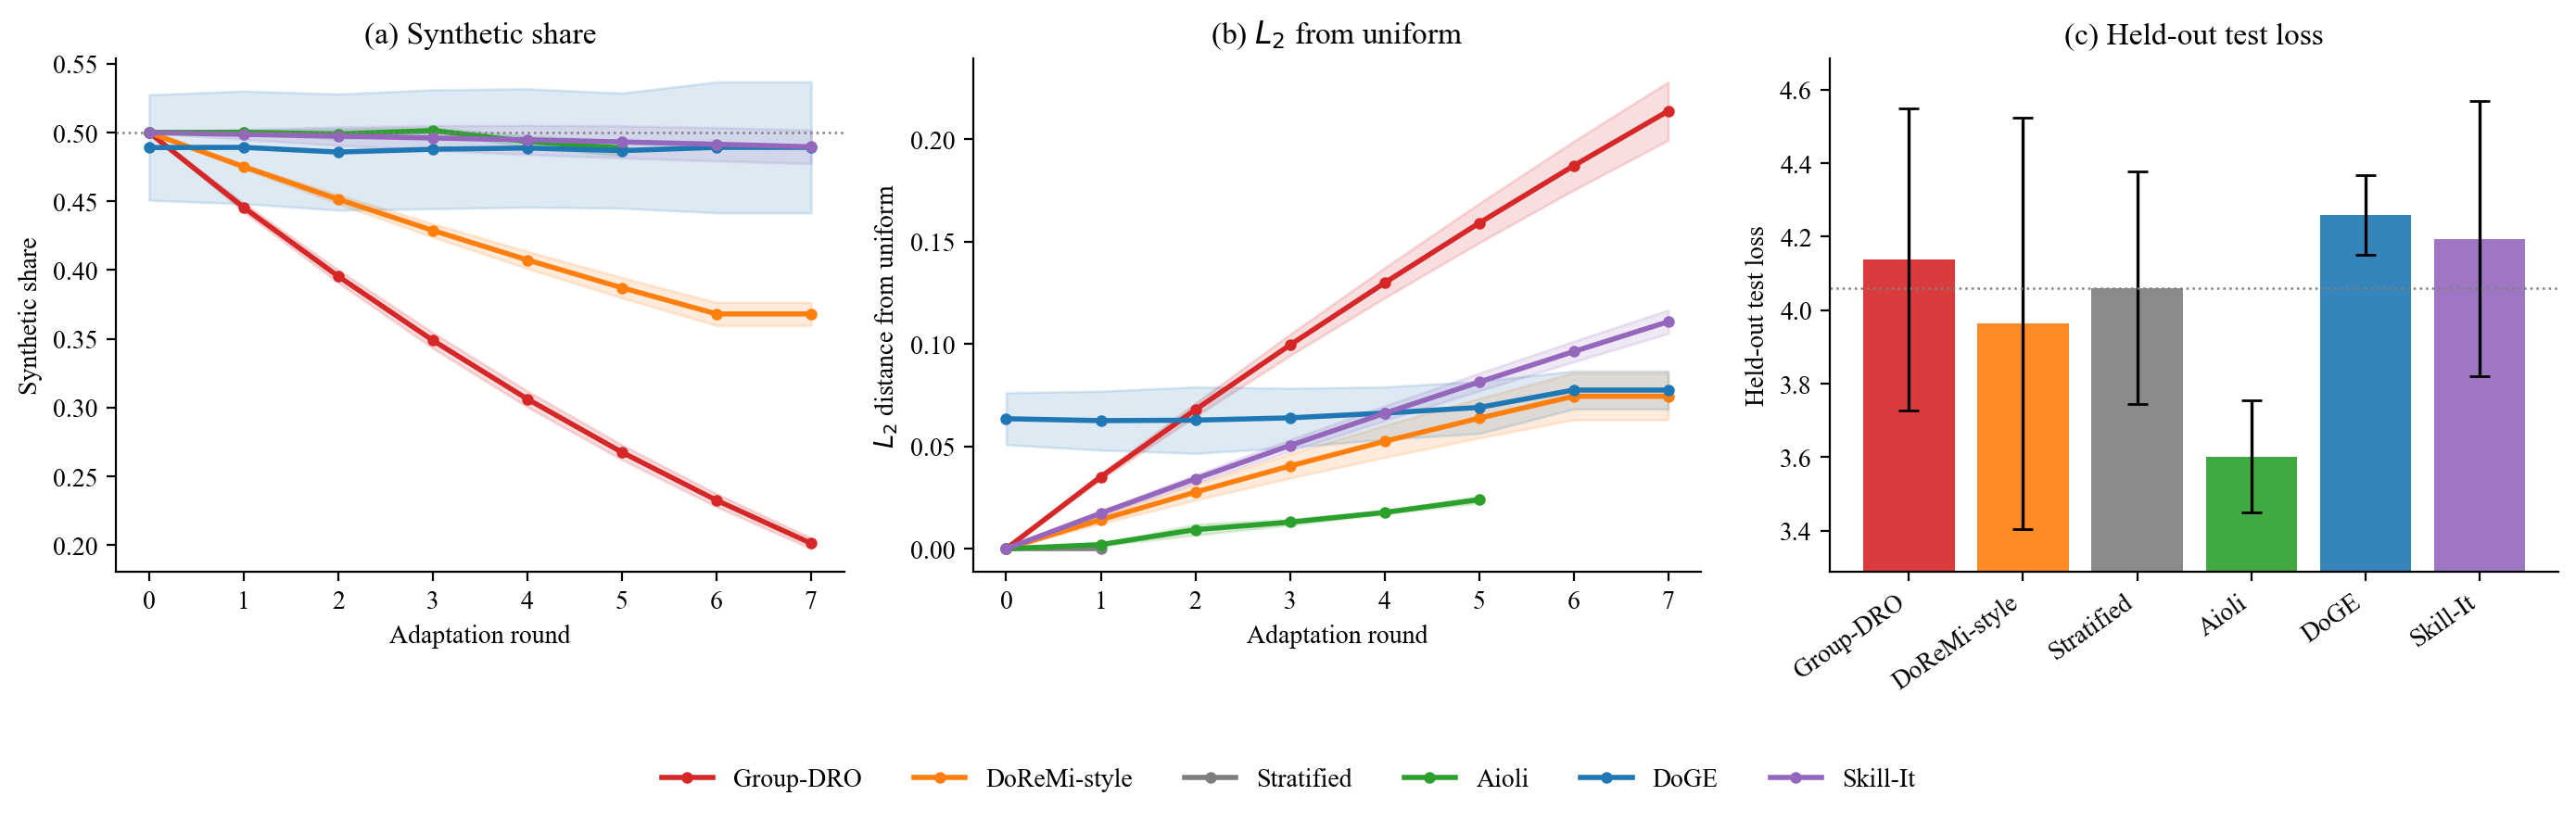
\includegraphics[width=0.80\linewidth]{figures/f_central.png}
\caption{Central result (bands are $\pm 1\sigma$ over seeds 0, 1, 2). (a) Synthetic share ($\sum p$ over the 9 synthetic domains) vs.\ reweighting round, start $=0.50$: loss-monotone methods move down, interaction and gradient estimators stay near uniform. (b) $L_2$ distance of the final mixture from uniform vs.\ round. (c) Held-out test loss by method (mean $\pm 1\sigma$ over seeds): Aioli has the lowest mean, but at $n=3$ on online-trained models this is a consistency read, not a ranking.}
\label{fig:central}
\end{figure}

\textbf{Which methods depart from uniform at this scale.} The policy split is clean and survives all three seeds (Figure~\ref{fig:central}a; per-seed in Appendix~\ref{app:perseed}). Methods keyed to loss drag the synthetic share down: Group-DRO reaches 0.20, the DoReMi-style variant 0.37. Aioli, Skill-It, and DoGE hardly leave their 0.50 start, sitting near 0.49. DoGE is the least stable, with its share wandering from 0.453 to 0.557 between seeds, a spread no other method shows. It traces to the self term in DoGE's score (Appendix~\ref{app:theory}), which leaks a domain's own loss whenever it outweighs the cross terms.

The $L_2$-from-uniform read (Figure~\ref{fig:central}b; computed per seed then averaged, Appendix~\ref{app:weights}) counts how much mass a method moves, direction aside: Group-DRO ($0.214$) $>$ Skill-It ($0.111$) $>$ DoGE ($0.077$) $\approx$ DoReMi-style ($0.074$) $>$ Aioli ($0.024$) $>$ Stratified ($0$). Skill-It is the oddity. Its share hardly moves, yet its $L_2$ lands second, because it churns weight inside each provenance class rather than across the line (Appendix~\ref{app:weights}).

\textbf{Does real-versus-synthetic change the ranking, and why.} Only the loss-monotone methods move much; the rest barely budge. Training pries open a loss gap between the two provenances, and the loss-movers chase it. Beforehand there's no gap to chase. At round 0 the provenances sit nearly tied (real 2.94, synthetic 2.90). One adaptation round later, real text is the high-loss side and templated synthetic the low-loss side, ending about one nat apart (final-round real 4.09, synthetic 3.06); we read the climb on real text as forgetting on the small fixed real shards (Figure~\ref{fig:valloss}). So it's not provenance the loss-movers chase. Group-DRO sheds low-loss real domains like Github and ArXiv and piles onto high-loss ones; what steers the weights is highest loss (Appendix~\ref{app:weights}).

\textbf{The held-out test loss, hedged.} Treat the quality read (Figure~\ref{fig:central}c; real and synthetic breakdown in Figure~\ref{fig:testloss-detail}; full means, sub-means, and per-seed values in Appendix~\ref{app:perseed}) cautiously. With $n=3$ it tells us about average behavior, not an ordering, because the models were scored after online training rather than a clean static retrain. Aioli has the lowest aggregate mean (3.60 nats) and beats DoGE and Skill-It on every seed; we take this as consistent with the mechanism, not a clean quality verdict, since online dynamics and Aioli's probe-driven trajectory are confounded with mixture choice. Against Stratified, DoReMi, and Group-DRO it lands within seed scatter, and no aggressive loss-mover pulls ahead of the uniform control by more than that scatter. Whichever method reallocates least wins the mean; the heaviest reallocators never clear uniform, matching Section~\ref{sec:mech}.

\section{Mechanism in brief}
\label{sec:mech}

What separates the families is how much the update's score leans on a domain's own loss. Group-DRO uses that loss straight. DoReMi instead measures excess loss against a reference, which dodges the pull toward irreducible noise. Aioli and DoGE ask, instead, how much training on a domain lowers loss elsewhere. Aioli's column sum stays purely cross-domain; DoGE's gradient inner product carries a self term that still tracks own loss. So DoGE escapes the loss-monotone pull only once cross-domain terms dominate, not by construction. This buys us an a-priori prediction (Appendix~\ref{app:theory}): a loss-monotone method drops the synthetic share exactly when real is the higher-loss provenance. When real turns hard and synthetic easy, loss-driven scores cut synthetic share where the interaction methods sit still, with sign $\mathrm{sign}(\overline{\ell}_{\mathrm{real}}-\overline{\ell}_{\mathrm{synth}})$, where $\overline{\ell}$ is the mean per-provenance validation loss. Derivation, loss-is-not-value decomposition, and out-of-sample corollary live in Appendix~\ref{app:theory}.

\section{Limitations and the compute floor}
\label{sec:limits}

\begin{figure}[t]
\centering
\includegraphics[width=\linewidth]{figures/f_scale_to_signal.pdf}
\caption{The compute floor: final synthetic share per method and tier (dots: seeds; bar: range; tick: mean). Below the floor the loss-monotone methods are seed-dominated (Group-DRO's seeds land at 0.253, 0.262, 0.996) or reversed (DoReMi-style); from the Intermediate tier on they sit tight below the 0.50 start, while the interaction and gradient methods stay near it.}
\label{fig:scale-signal}
\end{figure}

Two things deserve doubt: the protocol's signal and its budget. The quality read comes from online-trained models, not a static retrain, so it tangles the choice of mixture with online dynamics, plus probe overhead in Aioli's case; we hedge it rather than rank on it. For a verdict you'd retrain statically on each final mixture. Three seeds, one scenario, one model size (S2, 160M). The synthetic class is defined by instruction format rather than strictly by model generation (Section~\ref{sec:setup}), so provenance and template are confounded; the one synthetic slot whose loss overlaps the real band, Self-Instruct (4.03; Figure~\ref{fig:valloss}), is the human-written Dolly-15k. Split and $L_2$ ordering hold tight apart from DoGE, which we judge by its mean and update rule, not any single seed. The two cheaper tiers (Table~\ref{tab:flops}, Figure~\ref{fig:scale-signal}; Appendix~\ref{app:tiers}) locate a floor. The Intermediate tier ($1.2\times10^{16}$ FLOPs on pythia-70m) already reproduces the Full-tier split. At the Minimal tier ($2.5\times10^{14}$, a minutes-long smoke test) it falls apart: across seeds Group-DRO points nowhere on net (std 0.35) and DoReMi-style actually climbs, ending at 0.75. We read this as seed-dominated, not proven noise; at $n=3$ the two are hard to pull apart. The floor is the lowest budget where the loss-monotone methods agree in direction across seeds: Group-DRO's three Intermediate seeds land in $[0.234, 0.239]$, but at the Minimal tier they scatter to 0.996, 0.253, and 0.262. It sits between the two tiers. Both cheaper tiers run pythia-70m, so the floor is a budget effect at fixed model size, not a size effect; the Full tier (pythia-160m) only confirms it above, and an intermediate 160m point is untested. From roughly $10^{16}$ FLOPs the phenomenon reads clearly, three orders below a frontier run. Frontier compute isn't the requirement, just a modest floor. Whether the split survives past 160M we leave open.

\section{Conclusion}

Split a pool by provenance, pin the signal, read off the synthetic share: at 160M over three seeds, six data-mixing methods sort into two camps. Loss-monotone ones chase the hard real text downward; the rest sit near uniform, the steadiest (Aioli) posting the lowest mean held-out loss. Nobody reliably beats uniform; the protocol logs mixture choice, not quality, a reading already legible from about $10^{16}$ FLOPs (Section~\ref{sec:limits}).

\textbf{Using the probe.} To vet a new reweighter before any large sweep, run it beside Stratified and Group-DRO on a provenance-split pool at the Intermediate budget or above, over three seeds: about $1.1\times10^{17}$ FLOPs in all, less than one Full-tier run. Read each method's synthetic-share direction and its seed std. A share that falls with Group-DRO's, as tightly (std under 0.01), marks a loss-monotone policy; a share within scatter of 0.50 with a growing $L_2$, as for Skill-It, marks within-provenance reshuffling. Below the floor, where Group-DRO itself scatters, report the run as inconclusive, not as a null.

\section*{Acknowledgments}
We thank the Aioli authors for releasing their reference implementation, which our port follows, and EleutherAI for the open Pythia checkpoints.
% TODO(authors): add funding sources and compute provider before submission.

\section*{Ethics Statement}
We continue training small public checkpoints on public HuggingFace corpora (Appendix~\ref{app:repro}), used under their published terms for non-commercial research, and release code and aggregate statistics (losses, mixture weights, FLOPs), not raw text or model weights. Some synthetic corpora (e.g., Alpaca) are distilled from commercial models whose terms restrict downstream use; ShareGPT holds user-shared chatbot conversations that may contain personal information; the Pile contains web text of mixed copyright status, and our nine subsets exclude Books3. Our findings concern mixture choice only, not the safety of the resulting models.
% TODO(authors): add the LLM-usage disclosure if the venue requires one.

\clearpage
\bibliography{refs}
\bibliographystyle{colm2026_conference}

\newpage

\appendix

\section{Theoretical background}
\label{app:theory}

\paragraph{Setup.} Let domains be indexed by $i=1,\dots,k$, with mixture weights $p\in\Delta^{k-1}$ (the probability simplex) and per-domain validation loss $\ell_i(\theta)$. Online reweighting methods update $p$ across rounds and train on the mixture between updates. The methods we compare differ only in the score that drives a multiplicative-weights (exponentiated-gradient) update of the form
\begin{equation}
p_i^{(t+1)} \;\propto\; p_i^{(t)} \, \exp\!\big(\eta \, s_i^{(t)}\big),
\label{eq:mw}
\end{equation}
where $\eta$ is a step size and $s_i$ is the method-specific score. The families differ in whether $s_i$ is a function of $\ell_i$ alone.

\paragraph{Family 1: loss-monotone (Group-DRO, the DoReMi inner step).} Here the score is monotone increasing in a domain's own (excess) loss:
\begin{align}
\text{Group-DRO:}\quad & s_i = \ell_i - \tfrac{1}{k}\textstyle\sum_j \ell_j, \\
\text{DoReMi:}\quad & s_i = \big(\ell_i - \ell_i^{\mathrm{ref}}\big) - \tfrac{1}{k}\textstyle\sum_j \big(\ell_j - \ell_j^{\mathrm{ref}}\big),
\end{align}
where $\ell_i^{\mathrm{ref}}$ is a reference-model loss. Equation~\eqref{eq:mw} with the Group-DRO score is online mirror descent on the worst-case (distributionally robust) objective
\begin{equation}
\max_{p \in \Delta^{k-1}} \; \sum_{i=1}^{k} p_i \, \ell_i ,
\label{eq:dro}
\end{equation}
whose maximizer concentrates mass on $\arg\max_i \ell_i$ \citep{groupdro2020}. Plain worst-case (raw-loss) optimization therefore climbs toward the highest-loss domains, which on a heterogeneous pool are the noisiest, highest-irreducible-loss ones; our Group-DRO baseline is exactly this raw-loss objective. DoReMi differs in an important way: it scores the \emph{excess} loss over a reference, $\ell_i-\ell_i^{\mathrm{ref}}$, precisely so that a domain that is hard for everyone (high $\ell_i$ but also high $\ell_i^{\mathrm{ref}}$) does not dominate; the excess-loss centering is what counters the raw-loss pull toward irreducible noise \citep{doremi2023}. Our DoReMi-style proxy keeps the excess-loss form but, like Group-DRO, drops the joint min-max model step, so it sits between the two; this is why it moves the synthetic share down (to 0.37) less than raw Group-DRO (to 0.20). Its reference is a fixed pretrained base, provenance-neutral at the start, so subtracting it preserves the training-induced gap and the proxy stays in the loss-monotone family; a reference further trained on the pool would move off provenance-neutral and need not stay loss-monotone, so the grouping is contingent on the frozen reference.

\paragraph{Family 2: interaction / gradient (Aioli, DoGE).} Here the signal is cross-domain, not $\ell_i$. Aioli (Linear Mixing Optimization) models the loss dynamics as a linear mixing law,
\begin{equation}
\ell_i^{(t+1)} \;\approx\; \ell_i^{(t)} - \sum_{j} A_{ij}\, p_j ,
\qquad A_{ij} = \text{effect of training on } j \text{ on the loss of } i ,
\label{eq:aioli-law}
\end{equation}
with $A$ estimated by near-one-hot probe sweeps. The exploit step is exponentiated-gradient descent on the \emph{column sums} of $A$:
\begin{equation}
p_j^{(t+1)} \;\propto\; p_j^{(t)} \exp\!\Big(\eta \textstyle\sum_i A_{ij}\Big) .
\label{eq:aioli-egd}
\end{equation}
It upweights domains $j$ whose training most reduces the average loss (large column sum), not domains with high own loss. DoGE uses a first-order Taylor argument: a step on domain $j$ moves $\theta$ by $-\eta \nabla \ell_j$, and the change in the universal-generalization target $L_T$ (with gradient $g_T = \sum_i \nabla \ell_i$) is approximately $\eta \langle \nabla \ell_j, g_T \rangle$. So DoGE scores $j$ by the gradient inner product
\begin{equation}
s_j = \Big\langle \nabla \ell_j, \; \textstyle\sum_i \nabla \ell_i \Big\rangle ,
\label{eq:doge}
\end{equation}
the gradient-space analogue of Aioli's column sums \citep{aioli2024, doge2024}. Aioli's column sum is not a function of $\ell_j$ at all; DoGE's inner product expands into a self term $\lVert\nabla\ell_j\rVert^2$, correlated with domain $j$'s own loss, plus cross terms $\sum_{i\neq j}\langle\nabla\ell_j,\nabla\ell_i\rangle$, so it is not a function of $\ell_j$ alone but is not strictly free of it either. DoGE's near-uniform behavior here is conditional on the cross terms dominating, which holds empirically on this pool but is not guaranteed by the score.

\paragraph{Family 3: hybrid (Skill-It).} Skill-It learns a skills graph $A$ ($A_{ij} =$ effect of training skill $i$ on eval skill $j$), then applies the multiplicative-weights update
\begin{equation}
w_i^{(t+1)} \;\propto\; w_i^{(t)} \exp\!\Big(\eta \textstyle\sum_j A_{ij}\, \ell_j\Big),
\label{eq:skillit}
\end{equation}
the current per-skill loss \emph{weighted through the learned influence graph} \citep{skillit2023}. The loss enters, but only via which skills it helps, so the update is intermediate between the two families and, on this pool, reshuffles within rather than across the provenance boundary.

\paragraph{The a-priori prediction.} A loss-monotone update (Eq.~\eqref{eq:mw} with $s_i$ monotone in $\ell_i$) is forced toward the highest-loss provenance class; an interaction or gradient update (Eq.~\eqref{eq:aioli-egd}, Eq.~\eqref{eq:doge}) is not, because its move depends on column sums of $A$, not on $\ell$. Which provenance is higher-loss is an empirical input. On a provenance-split pool the two families therefore generically select different mixtures, and the sign of the synthetic-share movement equals
\begin{equation}
\mathrm{sign}\!\big(\overline{\ell}_{\mathrm{real}} - \overline{\ell}_{\mathrm{synth}}\big).
\label{eq:sign}
\end{equation}
Measured on the online-trained model, $\overline{\ell}_{\mathrm{real}} = 4.09 > \overline{\ell}_{\mathrm{synth}} = 3.06$ (final round), so the loss-movers reduce the synthetic share while the interaction methods stay near uniform. An out-of-sample corollary: on a homogeneous all-real pool with no provenance loss gap, the families should not split. This is a cheap, falsifiable control we reserve for follow-up work; until it is run we describe the protocol as a candidate instrument, and a confirmed non-split would establish it as a reusable one.

\paragraph{Loss is not value (our synthesis).} The DRO objective in Eq.~\eqref{eq:dro} targets $\ell_i$ (the worst case), but the quantity governing generalization is the transfer $\sum_i A_{ij}$ that Aioli and DoGE estimate (Eq.~\eqref{eq:aioli-egd}, Eq.~\eqref{eq:doge}); these coincide only if high loss implies high transfer, which is false in general. Decompose
\begin{equation}
\ell_i \;=\; H_i \;+\; \underbrace{(\ell_i - H_i)}_{\text{reducible gap}},
\label{eq:decomp}
\end{equation}
where $H_i$ is the irreducible entropy. A raw-loss method cannot separate the two terms, so it chases whichever provenance carries the higher loss whether or not that loss is reducible; here the real text becomes the high-loss provenance on the online-trained model and gets chased, even though high loss is not high value. DoReMi's excess-loss centering is the standard fix for exactly this failure of the raw-loss objective \citep{doremi2023}, and Aioli's own finding is adjacent but distinct: that prior methods set their mixing-law parameters inaccurately, so loss-based mixing-law fits are unreliable predictors of good mixtures, and no prior method consistently beats stratified sampling \citep{aioli2024}. That a datum's loss differs from its value for generalization is also the premise of data-valuation and influence work \citep{datashapley2019, less2024}, and selection signals keyed to the perplexity-to-downstream relationship rather than raw loss level reflect the same distinction \citep{thrush2025perplexitycorr}. We read ``loss is not value'' as our synthesis of these observations, not as a claim any of these papers makes verbatim. Our held-out test loss is consistent with it: the aggressive raw-loss movers do not beat the uniform baseline beyond seed noise, while the near-uniform interaction method (Aioli) has the lowest mean.

\section{Per-method weight evolution}
\label{app:weights}

\paragraph{$L_2$-from-uniform ordering and per-domain concentrations.} The $L_2$ distance of the final mixture from uniform at the final round is Group-DRO $0.214 >$ Skill-It $0.111 >$ DoGE $0.077 \approx$ DoReMi-style $0.074 >$ Aioli $0.024 >$ Stratified $0$. Skill-It is the informative case: its synthetic share barely moves (0.49), yet its $L_2$ is second highest, because it reshuffles weight within each provenance class rather than across the real/synthetic boundary, so the synthetic-share number alone would mislabel it as inert. The per-domain weights are consistent (uniform $=0.0556$): Group-DRO concentrates on high-loss real domains (Pile-CC 0.164, OpenWebText2 0.150) and starves easy synthetic ones (Code-Alpaca 0.004), while also trimming lower-loss real domains (Github 0.027, ArXiv 0.030), so the signal is highest-loss, not real as such; Aioli stays in a tight band (0.048 to 0.068).

The final per-domain weights confirm the reading. Figure~\ref{fig:finalweights} gives them as a method-by-domain heatmap and Figure~\ref{fig:finalweights-detail} as grouped bars with per-seed error bands: Group-DRO concentrates aggressively on high-loss real domains and starves easy synthetic ones, Aioli stays in a tight near-uniform band, and DoGE is near-uniform but the noisiest. Figure~\ref{fig:valloss} shows the Aioli per-domain validation-loss trajectories, where real domains sit high (mean 4.09) and synthetic domains sit low (mean 3.06), the empirical input that fixes the sign in Eq.~\eqref{eq:sign}.

\begin{figure}[t]
\centering
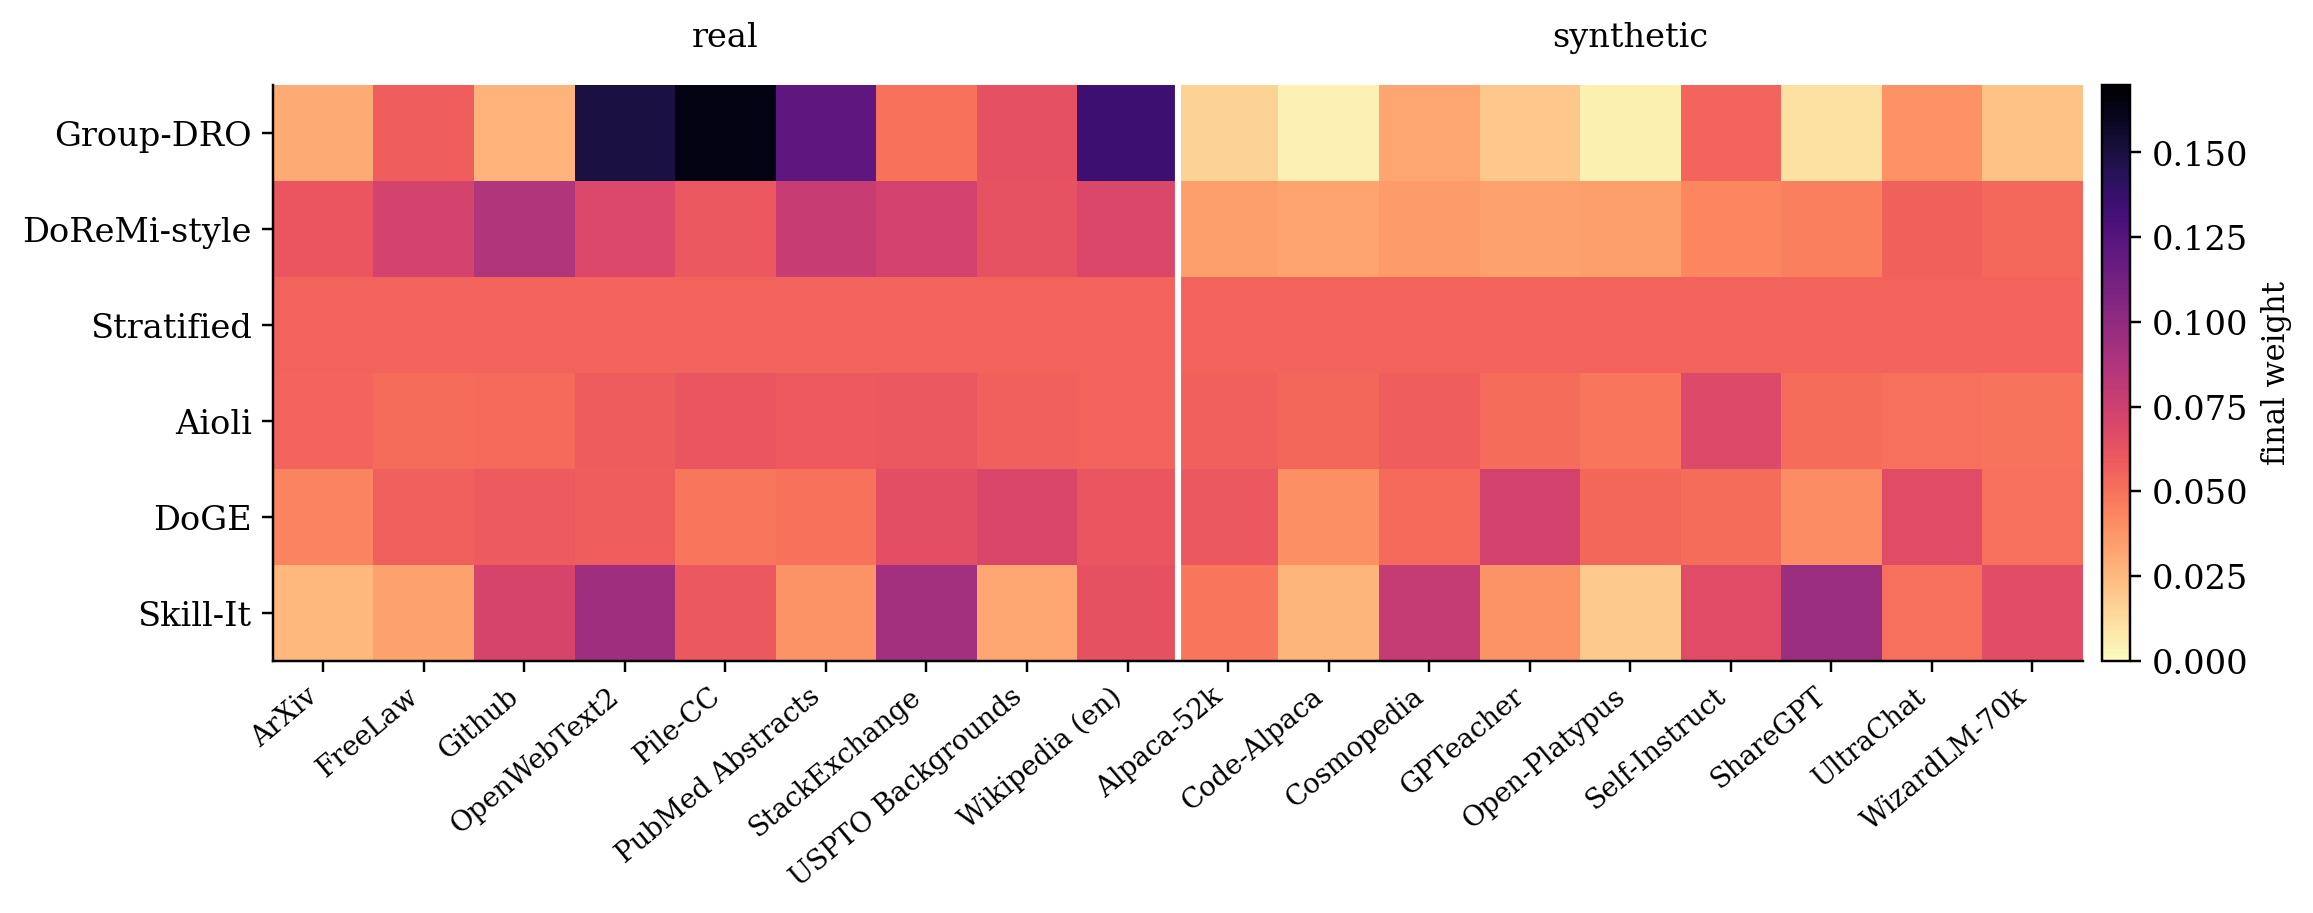
\includegraphics[width=\linewidth]{figures/f_finalweights.png}
\caption{Final per-domain weights as a method-by-domain heatmap (mean over seeds; uniform $=0.0556$), the real block left of the divider and the synthetic block right. Group-DRO is the most concentrated (dark cells on high-loss real domains, near-zero on easy synthetic ones); Aioli is the flattest non-trivial method.}
\label{fig:finalweights}
\end{figure}

\begin{figure}[t]
\centering
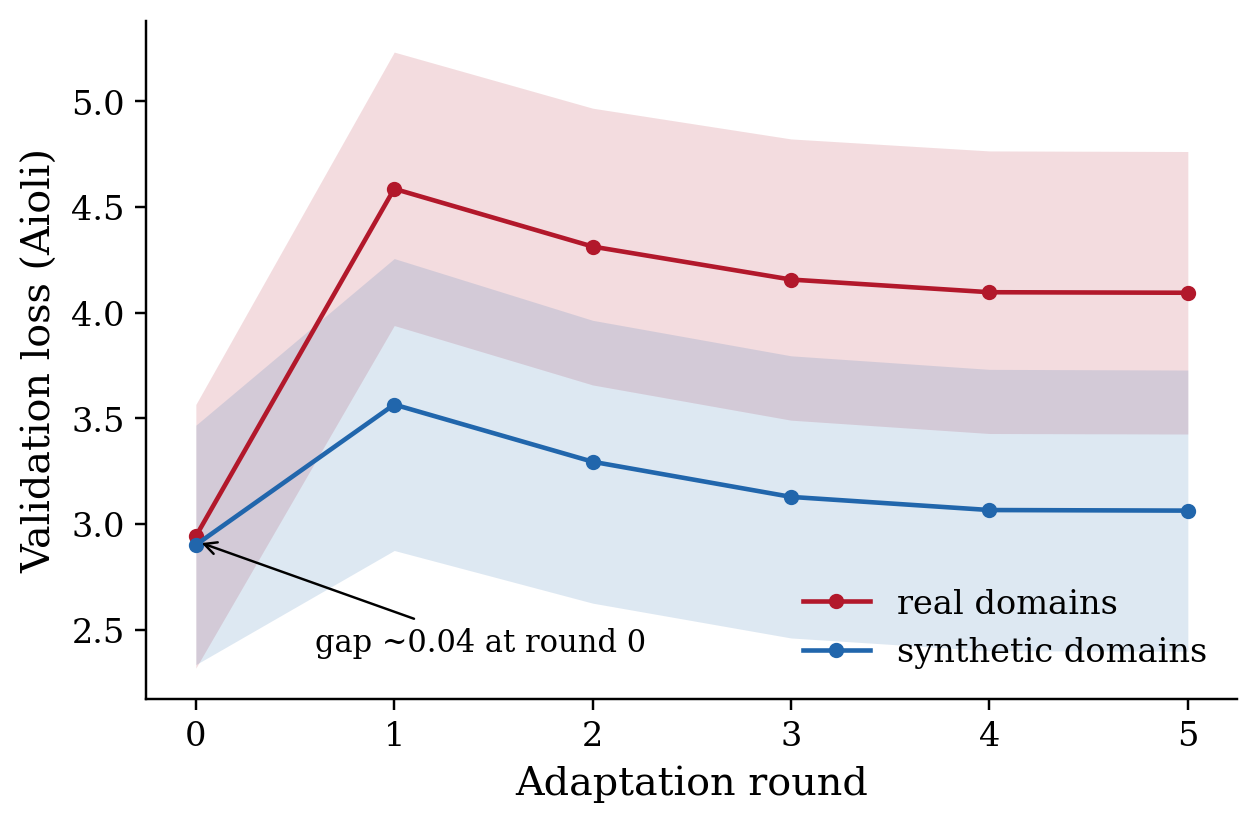
\includegraphics[width=0.66\linewidth]{figures/f_valloss.png}
\caption{Per-provenance validation loss across rounds (Aioli run; line is the class mean, band the per-class spread). At round 0, the base checkpoint, real and synthetic are nearly tied (2.94 vs 2.90, gap 0.04); the gap opens inside the first adaptation round and settles near one nat (final-round real 4.09, synthetic 3.06), the real-domain rise consistent with forgetting on the small fixed real shards. At the final round the three lowest domains are synthetic (Code-Alpaca 2.00, Open-Platypus 2.23, ShareGPT 2.63) and the four highest real (Pile-CC 4.90, OpenWebText2 4.78, Wikipedia 4.62, PubMed 4.49), with Github (real, 2.90) and Self-Instruct (synthetic, 4.03) overlapping, so the split is systematic, not strict. This training-induced ordering is the empirical input that fixes the sign in Eq.~\eqref{eq:sign}.}
\label{fig:valloss}
\end{figure}

\begin{figure}[t]
\centering
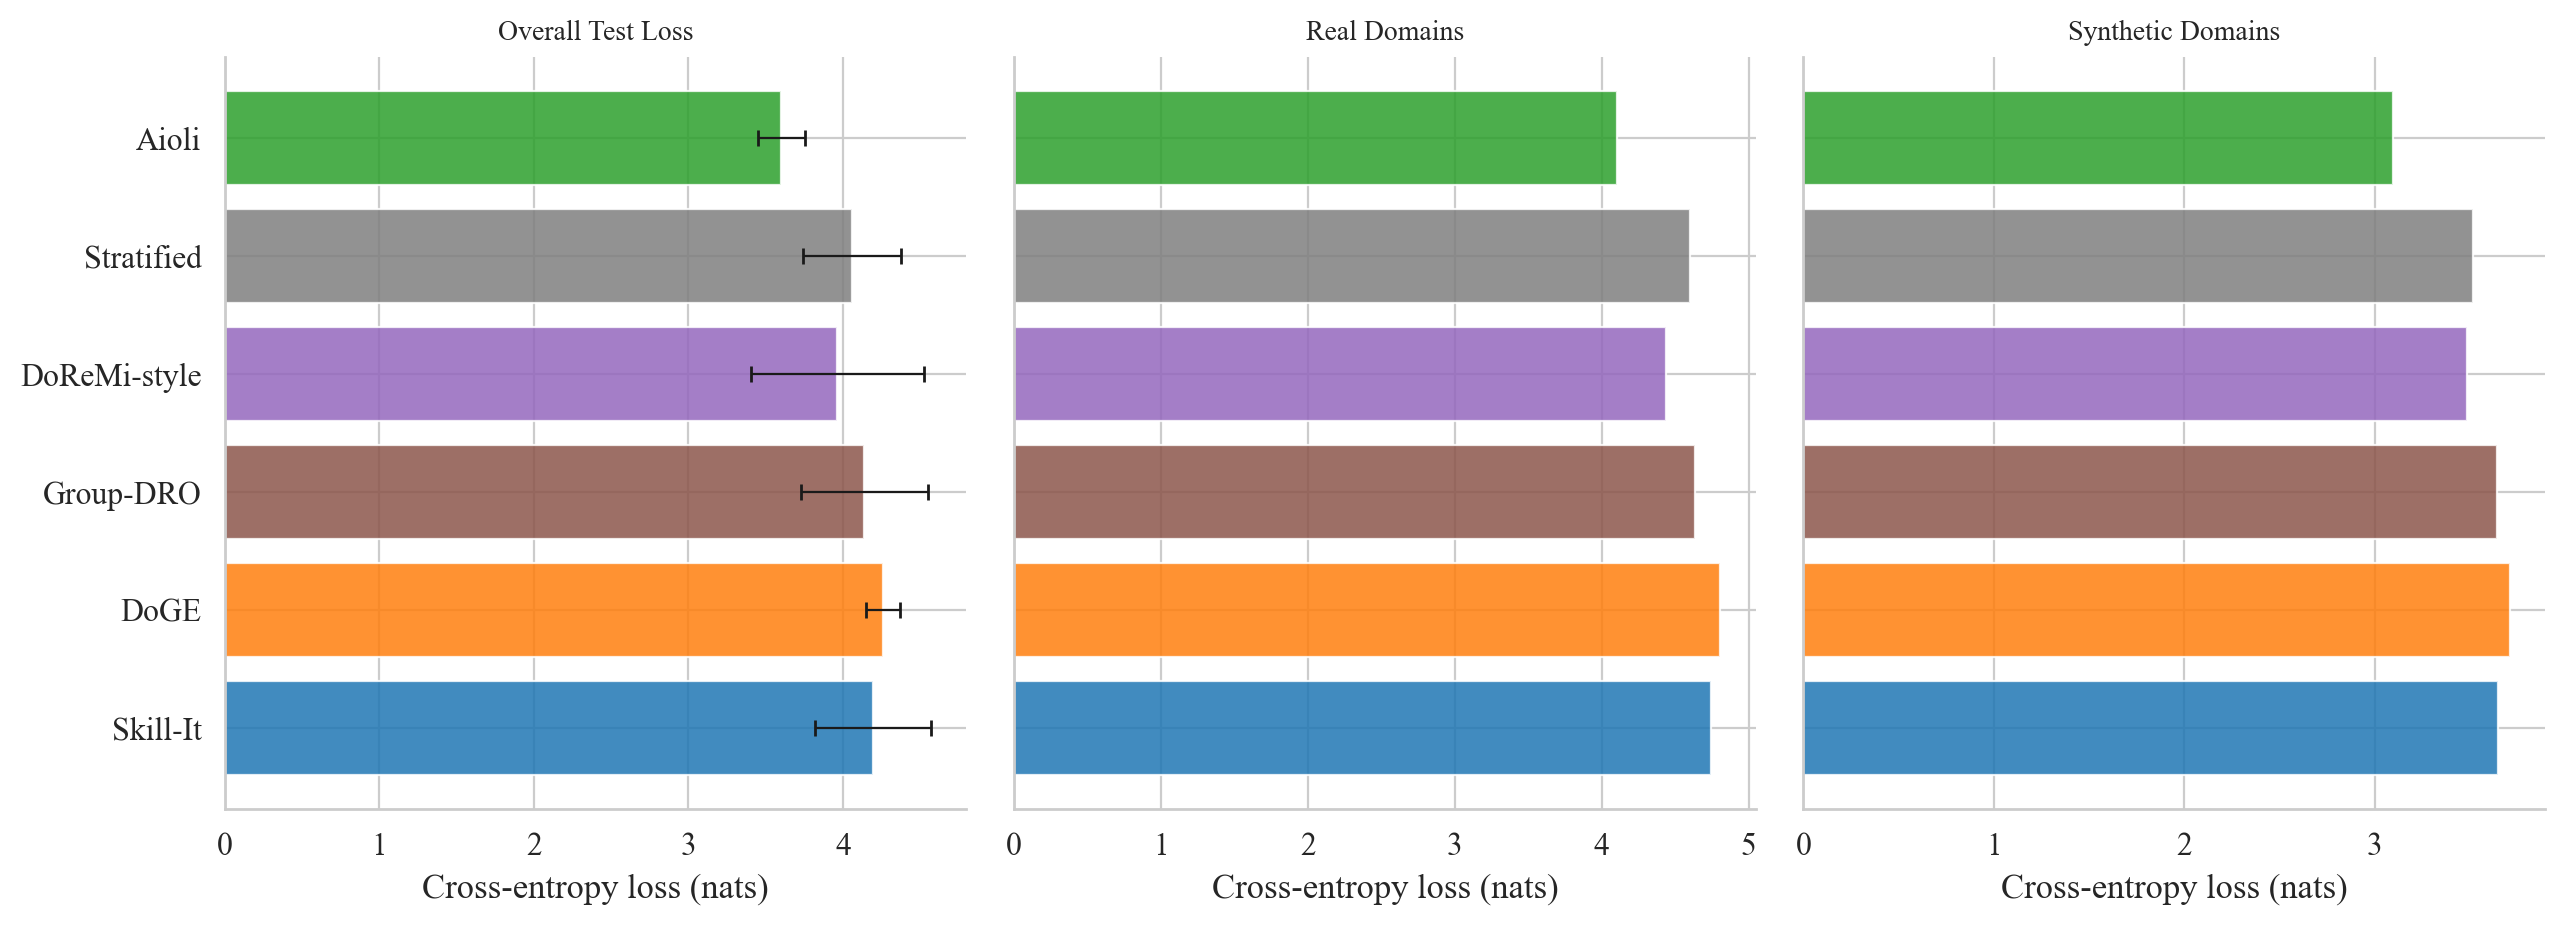
\includegraphics[width=\linewidth]{figures/HEAVY_S2_9R_9S_test_loss.png}
\caption{Held-out test loss disaggregated by provenance (Pythia-160m, Full tier, seeds 0, 1, 2). \emph{Left}: aggregate mean cross-entropy loss (nats) over all 18 domains, with $\pm 1\sigma$ error bars across seeds. \emph{Centre}: mean over the 9 real Pile subsets. \emph{Right}: mean over the 9 synthetic instruction domains. Aioli achieves the lowest aggregate mean (3.60) and beats DoGE and Skill-It on all three seeds; it does not reliably beat Stratified, DoReMi-style, or Group-DRO at $n{=}3$, consistent with the average-case reading in Section~\ref{sec:mech}. The consistent per-provenance gap, real domains scoring roughly one nat higher than synthetic for every method, independently confirms the training-induced loss ordering of Figure~\ref{fig:valloss}. The aggressive loss-movers (Group-DRO 4.14, DoReMi-style 3.96) do not improve over the uniform control (Stratified 4.06) in the aggregate mean, consistent with the mechanism in Section~\ref{sec:mech}: chasing the high-loss real provenance reallocates mass but does not lower the balanced-pool test loss.}
\label{fig:testloss-detail}
\end{figure}

\begin{figure}[t]
\centering
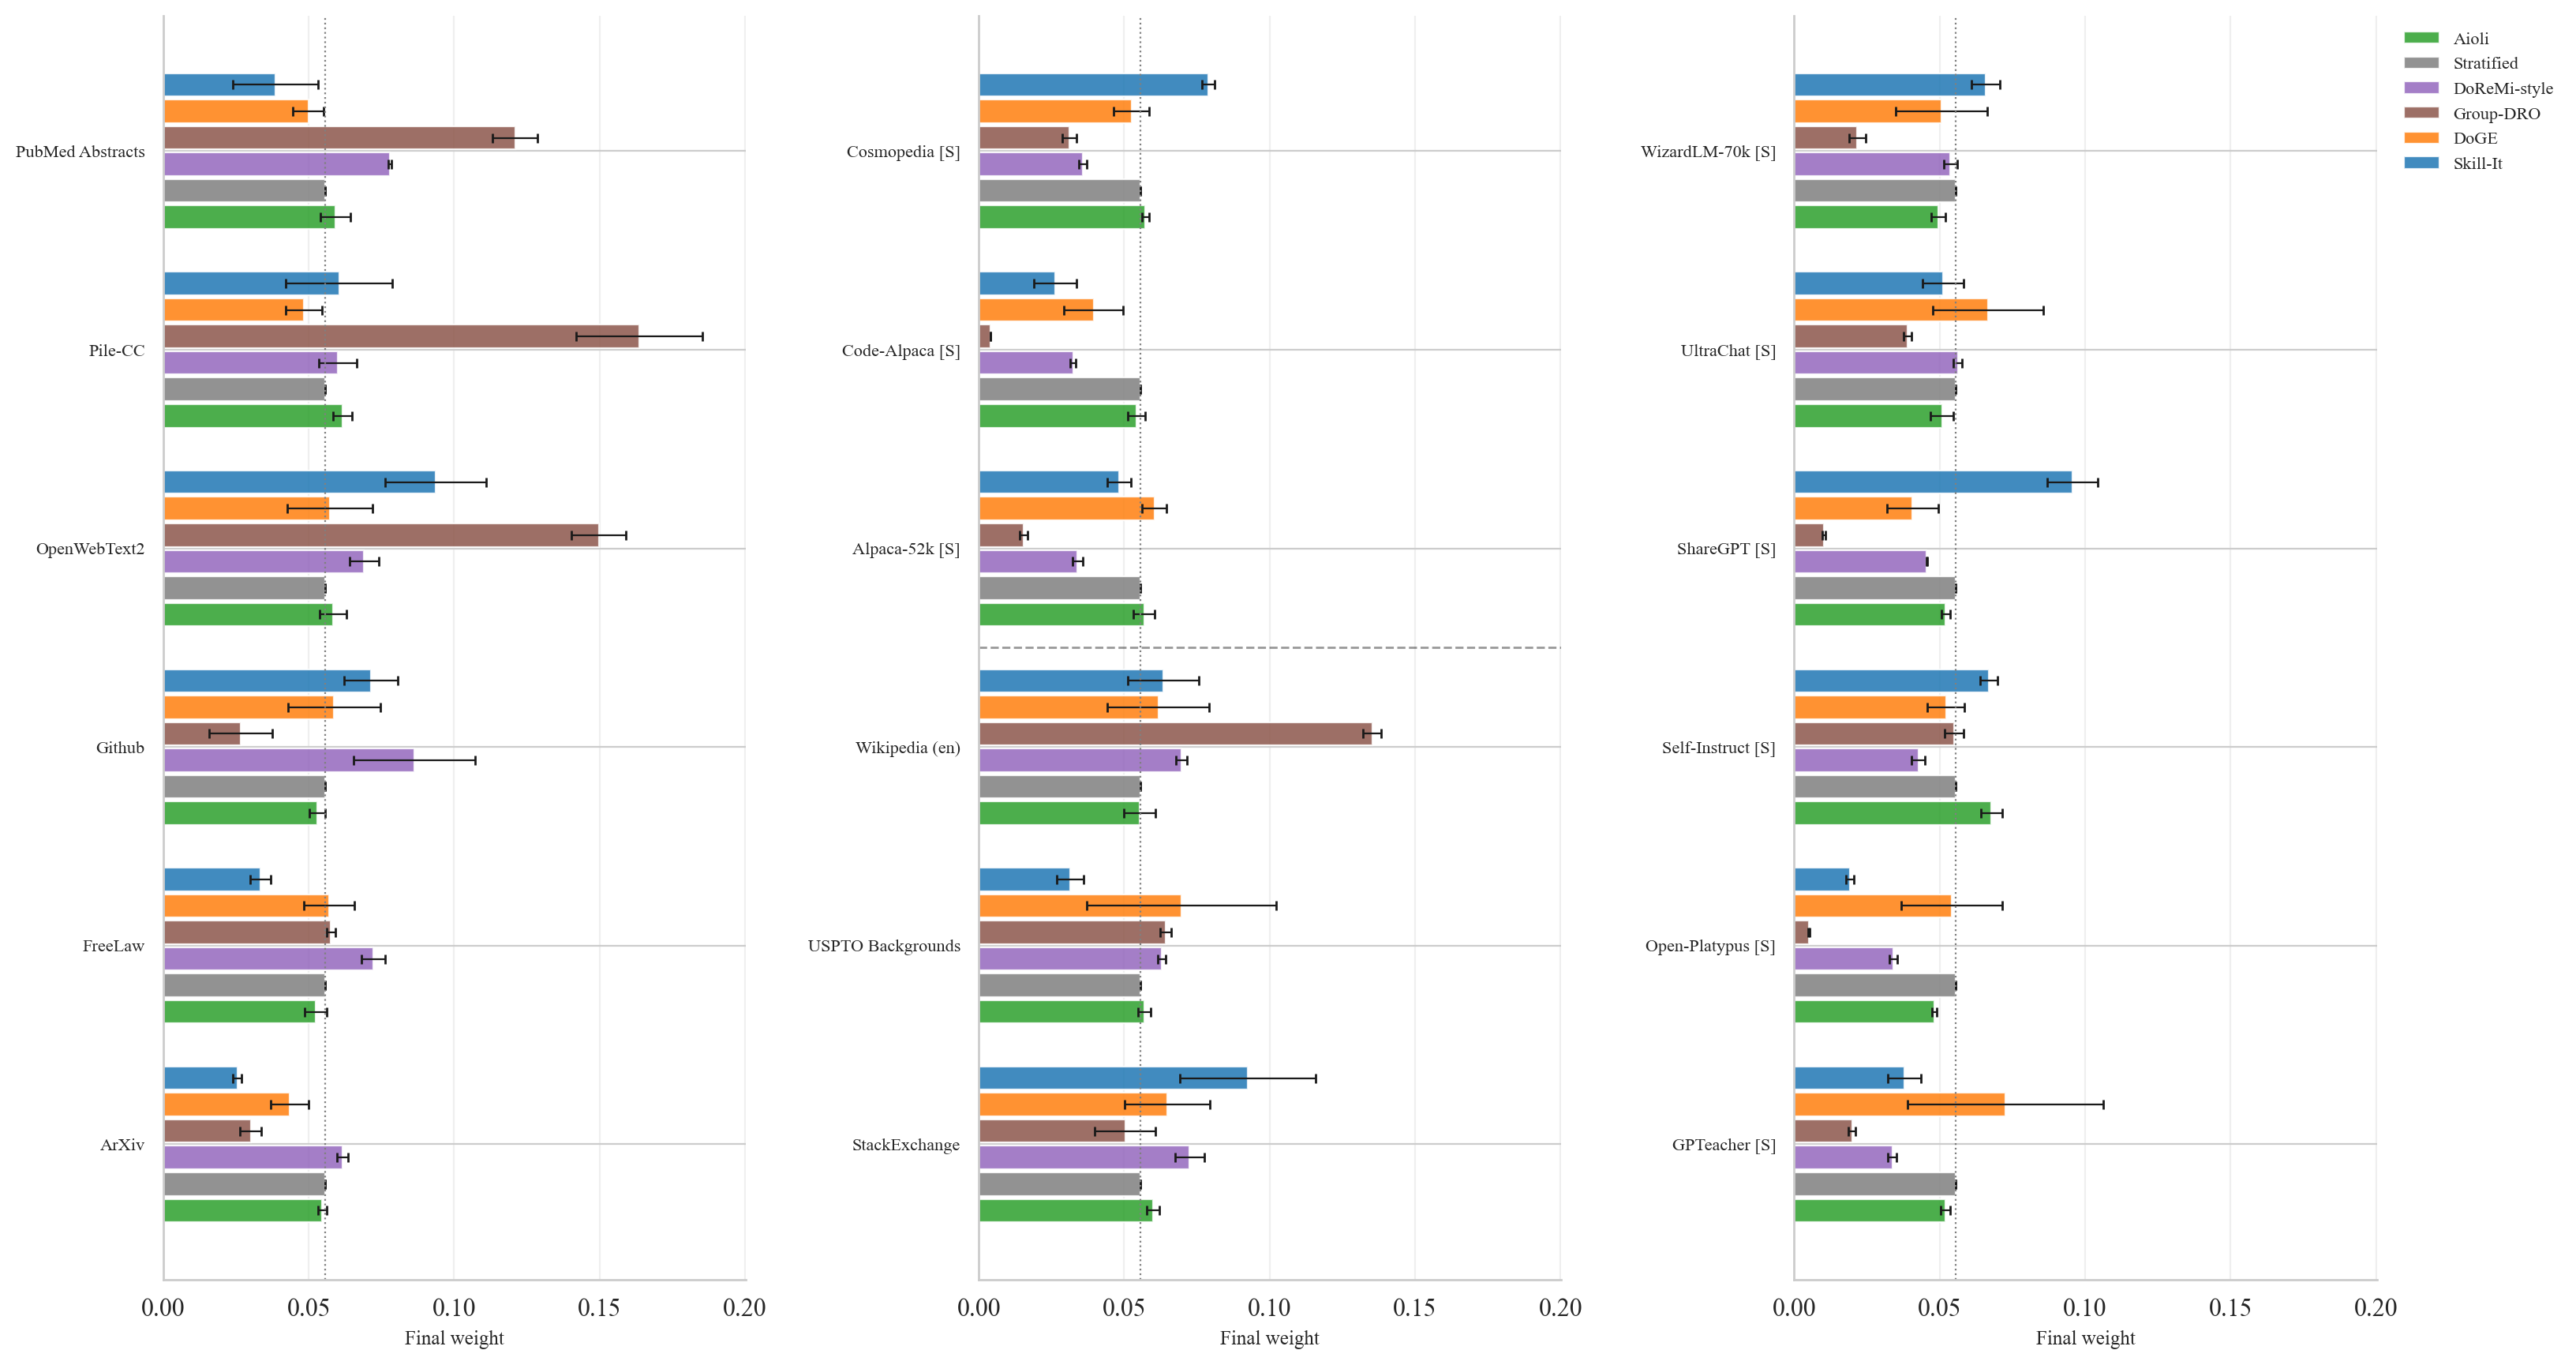
\includegraphics[width=\linewidth]{figures/HEAVY_S2_9R_9S_final_weights.png}
\caption{Final per-domain mixture weights as a grouped horizontal bar chart (mean $\pm 1\sigma$ over seeds 0, 1, 2; uniform $= 0.0\overline{5}$), complementing the heatmap of Figure~\ref{fig:finalweights} with per-method error bars. Domains are sorted alphabetically within each provenance class. Group-DRO concentrates on the highest-loss real domains (Pile-CC 0.164, OpenWebText2 0.150) and drives several synthetic domains near zero (Code-Alpaca 0.004), while also trimming the low-loss real domains (Github 0.027, ArXiv 0.030): the discriminating signal is per-domain loss magnitude, not provenance category per se. DoReMi-style shows the same directional pattern at attenuated magnitude. Aioli stays in a narrow band around uniform (approximately 0.04 to 0.07) with small cross-seed variance. Skill-It is the most informative case: individual domains within each provenance class deviate substantially from uniform, ShareGPT elevated in the synthetic block and OpenWebText2 and StackExchange elevated in the real block, yet the total mass on each class remains near 0.50, the within-class reshuffling behavior visible at the domain level (see also Figure~\ref{fig:we-skillit}).}
\label{fig:finalweights-detail}
\end{figure}

\begin{figure}[t]
\centering
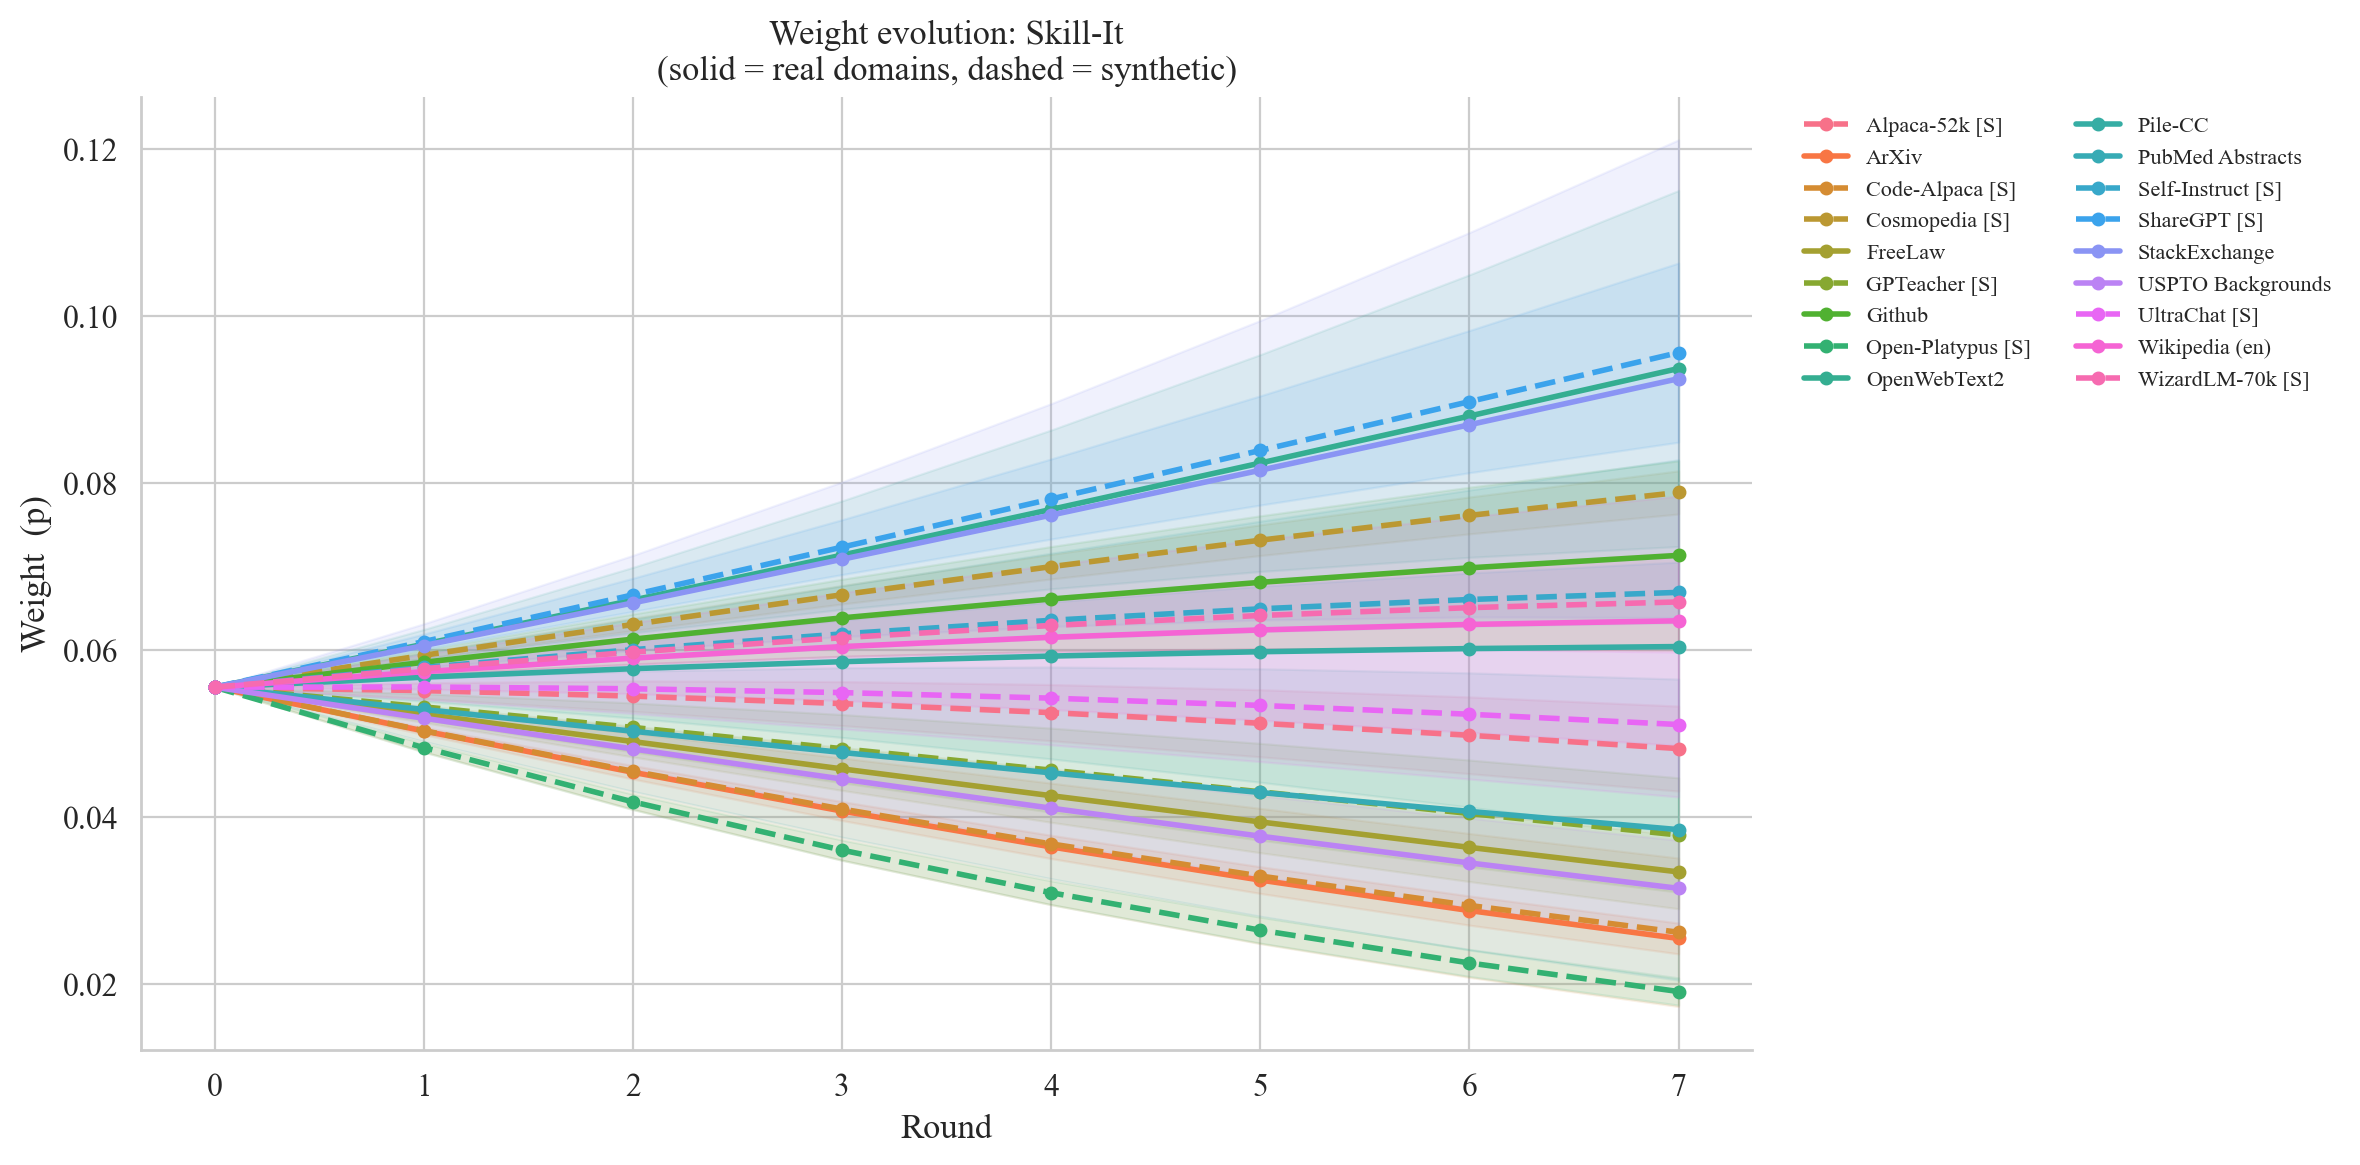
\includegraphics[width=0.9\linewidth]{figures/HEAVY_S2_9R_9S_Skill-It_weight_evolution.png}
\caption{Skill-It per-domain weight trajectories across reweighting rounds (solid lines $=$ real domains; dashed lines $=$ synthetic domains; shaded bands $=$ $\pm 1\sigma$ over seeds 0, 1, 2). Skill-It shows bidirectional, within-class movement: some synthetic domains gain weight (Cosmopedia, Self-Instruct) while others fall (Code-Alpaca, GPTeacher), and a symmetric pattern holds within the real class. The total synthetic share stays near 0.49 throughout even as the $L_2$ distance from uniform reaches 0.111 (second only to Group-DRO), making Skill-It the method that moves most without crossing the provenance boundary. This is the empirical signature of the graph-weighted update (Appendix~\ref{app:theory}, Family 3): the learned influence graph $A$ discriminates among domains within a provenance class more sharply than across the provenance boundary at this scale. The wider inter-seed bands on certain domains (StackExchange, OpenWebText2) indicate that specific within-class rankings are less seed-stable than the family-level synthetic-share result, consistent with the observations in Section~\ref{sec:mech}.}
\label{fig:we-skillit}
\end{figure}

\section{Complete per-seed tables}
\label{app:perseed}

Table~\ref{tab:testloss} gives the aggregate held-out test loss with real/synthetic sub-means, Table~\ref{tab:perseed-share} the per-seed synthetic-share endpoints, and Table~\ref{tab:perseed-test} the per-seed aggregate test loss.

\begin{table}[t]
\centering
\small
\caption{Held-out test loss (lower is better), aggregate mean over 18 domains, mean $\pm$ std over 3 seeds, then real-only and synthetic-only sub-means. Read as an average-case signal at $n=3$, not a ranking.}
\label{tab:testloss}
\begin{tabular}{llll}
\toprule
Method & test loss (mean $\pm$ std) & real & synth \\
\midrule
Aioli & $3.60 \pm 0.15$ & 4.10 & 3.10 \\
DoReMi-style & $3.96 \pm 0.56$ & 4.44 & 3.49 \\
Stratified & $4.06 \pm 0.32$ & 4.60 & 3.52 \\
Group-DRO & $4.14 \pm 0.41$ & 4.63 & 3.64 \\
Skill-It & $4.19 \pm 0.37$ & 4.74 & 3.65 \\
DoGE & $4.26 \pm 0.11$ & 4.81 & 3.71 \\
\bottomrule
\end{tabular}
\end{table}

The synthetic-share split is tight across seeds for every method except DoGE, whose share swings from 0.453 to 0.557. The test-loss read is the fragile one. Aioli has the lowest mean and beats DoGE and Skill-It on all three seeds, so the claim ``Aioli has the best mean test loss and reliably beats DoGE and Skill-It'' is defensible. But Aioli beats Stratified on only two of three seeds (Stratified is lower on seed 2, 3.62 vs 3.67) and is mixed against DoReMi and Group-DRO, so it does \emph{not} reliably beat Stratified, DoReMi, or Group-DRO; we do not claim it is the only method to beat the uniform control or trains a definitively better model. The aggressive loss-movers are narrower still: neither beats uniform by more than noise (Group-DRO is worse on the mean, 4.14 vs 4.06; DoReMi-style lower by only 0.10 with std 0.56, inside the scatter). The consistent real-versus-synthetic gap across every method (real about 4.1 to 4.8, synthetic about 3.1 to 3.7) independently confirms that the templated synthetic text is the easier (lower-loss) provenance on the online-trained models, consistent with the training-induced gap of Figure~\ref{fig:valloss}.

\begin{table}[t]
\centering
\small
\caption{Per-seed synthetic-share endpoints (start $=0.50$).}
\label{tab:perseed-share}
\begin{tabular}{lllll}
\toprule
Method & seed 0 & seed 1 & seed 2 & mean \\
\midrule
Group-DRO & 0.197 & 0.201 & 0.206 & 0.20 \\
DoReMi-style & 0.376 & 0.372 & 0.356 & 0.37 \\
Stratified & 0.500 & 0.500 & 0.500 & 0.50 \\
Aioli & 0.482 & 0.496 & 0.488 & 0.49 \\
Skill-It & 0.503 & 0.473 & 0.492 & 0.49 \\
DoGE & 0.557 & 0.453 & 0.458 & 0.49 \\
\bottomrule
\end{tabular}
\end{table}

\begin{table}[t]
\centering
\small
\caption{Per-seed aggregate held-out test loss (lower is better).}
\label{tab:perseed-test}
\begin{tabular}{lllll}
\toprule
Method & seed 0 & seed 1 & seed 2 & mean $\pm$ std \\
\midrule
Aioli & 3.39 & 3.74 & 3.67 & $3.60 \pm 0.15$ \\
DoReMi-style & 3.64 & 3.50 & 4.75 & $3.96 \pm 0.56$ \\
Stratified & 4.24 & 4.33 & 3.62 & $4.06 \pm 0.32$ \\
Group-DRO & 4.55 & 4.28 & 3.58 & $4.14 \pm 0.41$ \\
DoGE & 4.41 & 4.19 & 4.17 & $4.26 \pm 0.11$ \\
Skill-It & 3.68 & 4.36 & 4.55 & $4.19 \pm 0.37$ \\
\bottomrule
\end{tabular}
\end{table}

\section{Cross-tier results: the compute floor}
\label{app:tiers}

We run all three tiers of Table~\ref{tab:flops} over the same three seeds. The two pythia-70m tiers are not throwaway smoke tests; they locate where on the compute axis the loss-monotone split becomes legible. Figure~\ref{fig:tier-share} plots the synthetic-share trajectories at each budget, Figure~\ref{fig:scale-signal} (Section~\ref{sec:limits}) shows every seed's endpoint at each budget, and three tables give the numbers: final synthetic share (Table~\ref{tab:tier-share}), held-out test loss (Table~\ref{tab:tier-test}), and per-seed share at the two cheaper tiers (Table~\ref{tab:tier-perseed}).

The directional pattern holds above a floor and disappears below it. At the Full ($2.3\times10^{17}$ FLOPs) and Intermediate ($1.2\times10^{16}$) the loss-monotone family pulls the synthetic share down (Group-DRO to 0.20 and 0.24, DoReMi-style to 0.37 and 0.37) and the interaction and gradient methods stay near uniform. At the Minimal tier ($2.5\times10^{14}$, a minutes-long run on pythia-70m) the split is absent. Group-DRO ends at 0.50 with a seed std of 0.35, and the per-seed values explain why: one seed drives the synthetic share to 0.996 while the other two send it down (Table~\ref{tab:tier-perseed}). DoReMi-style runs the wrong way, ending at 0.75; its reversal is consistent across all three seeds (0.545, 0.850, 0.864), so below the floor it does not simply turn noisy the way Group-DRO does but enters a different regime, plausibly from extreme undertraining and fewer adaptation rounds. The seed std of the final share collapses with compute (Figure~\ref{fig:scale-signal}; Table~\ref{tab:tier-share}), Group-DRO from 0.35 at the Minimal tier to under 0.01 by the Intermediate tier, so beneath the floor the loss-monotone direction is unreliable, whether through incoherent scatter (Group-DRO) or coherent reversal (DoReMi-style). A minimum budget is necessary to read the split, but a small one, about $10^{16}$ FLOPs, three orders below a frontier run.

The held-out test loss needs the budget too (Table~\ref{tab:tier-test}). At the Minimal tier the 70m models are badly undertrained, losses of 7 to 10 nats with seed std up to 1.9, so no quality signal survives. At the Intermediate tier the six methods are statistically indistinguishable, all between 3.70 and 3.79; the Aioli-lowest-mean result (3.60 against a next-best 3.96) is a Full-tier effect. The quality read, like the directional split, sharpens only with compute, which is why we hedge it even at the Full tier.

\begin{figure}[t]
\centering
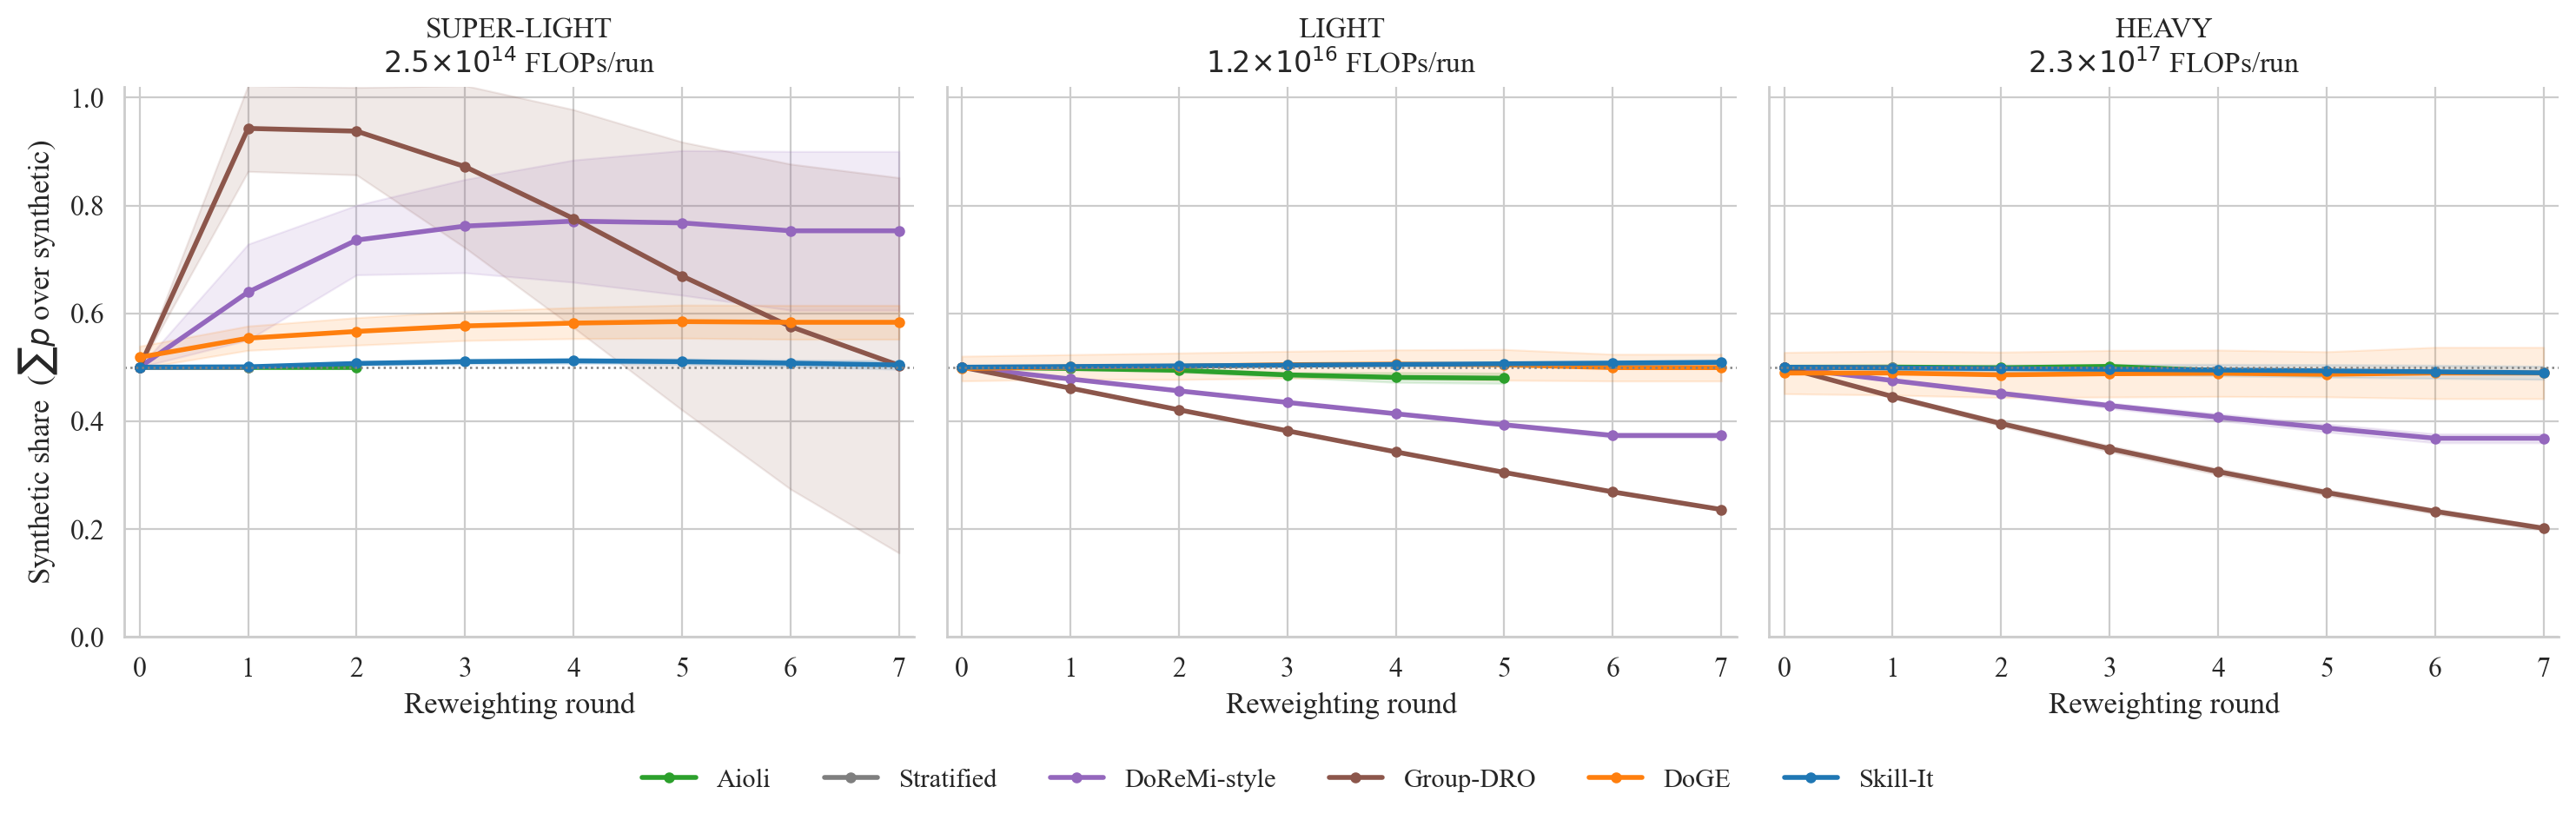
\includegraphics[width=\linewidth]{figures/f_tier_share_panels.png}
\caption{Synthetic-share trajectories at the three compute tiers (all methods, $\pm 1\sigma$ over seeds 0, 1, 2; start 0.50). At the Minimal tier the loss-monotone methods do not separate cleanly: Group-DRO spikes toward the synthetic class then collapses with a wide seed band, and DoReMi-style climbs to 0.75. From the Intermediate tier on, the split is the clean Full-tier pattern, loss-monotone methods down and the rest near uniform.}
\label{fig:tier-share}
\end{figure}

\begin{table}[t]
\centering
\small
\caption{Final synthetic share by tier (mean $\pm$ std over seeds 0, 1, 2; start 0.50). The loss-monotone split (Group-DRO, DoReMi-style move down) is present at the Intermediate and Full tiers but absent at the Minimal tier, where Group-DRO has no net direction (std 0.35) and DoReMi-style reverses. Interaction and gradient methods stay near 0.50 at every tier.}
\label{tab:tier-share}
\begin{tabular}{lccc}
\toprule
Method & Minimal & Intermediate & Full \\
 & ($2.5\times10^{14}$) & ($1.2\times10^{16}$) & ($2.3\times10^{17}$) \\
\midrule
Group-DRO & $0.50 \pm 0.35$ & $0.24 \pm 0.00$ & $0.20 \pm 0.00$ \\
DoReMi-style & $0.75 \pm 0.15$ & $0.37 \pm 0.00$ & $0.37 \pm 0.01$ \\
Aioli & $0.50 \pm 0.00$ & $0.48 \pm 0.01$ & $0.49 \pm 0.01$ \\
DoGE & $0.58 \pm 0.03$ & $0.50 \pm 0.03$ & $0.49 \pm 0.05$ \\
Skill-It & $0.50 \pm 0.01$ & $0.51 \pm 0.01$ & $0.49 \pm 0.01$ \\
Stratified & $0.50 \pm 0.00$ & $0.50 \pm 0.00$ & $0.50 \pm 0.00$ \\
\bottomrule
\end{tabular}
\end{table}

\begin{table}[t]
\centering
\small
\caption{Held-out test loss by tier (aggregate over 18 domains, mean $\pm$ std over seeds; lower is better). Minimal-tier 70m models are badly undertrained, so no quality signal survives; at the Intermediate tier the methods are within scatter (3.70 to 3.79); the Aioli-lowest-mean result is a Full-tier effect.}
\label{tab:tier-test}
\begin{tabular}{lccc}
\toprule
Method & Minimal & Intermediate & Full \\
\midrule
Aioli & $7.37 \pm 0.77$ & $3.70 \pm 0.00$ & $3.60 \pm 0.15$ \\
DoReMi-style & $9.54 \pm 1.88$ & $3.79 \pm 0.04$ & $3.96 \pm 0.56$ \\
Stratified & $7.33 \pm 0.64$ & $3.72 \pm 0.02$ & $4.06 \pm 0.32$ \\
Group-DRO & $8.57 \pm 1.35$ & $3.79 \pm 0.01$ & $4.14 \pm 0.41$ \\
DoGE & $7.50 \pm 1.01$ & $3.74 \pm 0.02$ & $4.26 \pm 0.11$ \\
Skill-It & $7.68 \pm 0.18$ & $3.70 \pm 0.01$ & $4.19 \pm 0.37$ \\
\bottomrule
\end{tabular}
\end{table}

\begin{table}[t]
\centering
\small
\caption{Per-seed final synthetic share at the two cheaper tiers (start 0.50). At the Minimal tier the loss-monotone methods are seed-dominated: Group-DRO sends one seed to 0.996 (toward synthetic) and two down, and DoReMi-style runs up on two of three. By the Intermediate tier the same methods are tight and pointed down.}
\label{tab:tier-perseed}
\begin{tabular}{lcccccc}
\toprule
 & \multicolumn{3}{c}{Minimal} & \multicolumn{3}{c}{Intermediate} \\
\cmidrule(lr){2-4}\cmidrule(lr){5-7}
Method & seed 0 & seed 1 & seed 2 & seed 0 & seed 1 & seed 2 \\
\midrule
Group-DRO & 0.996 & 0.253 & 0.262 & 0.234 & 0.239 & 0.235 \\
DoReMi-style & 0.545 & 0.850 & 0.864 & 0.376 & 0.368 & 0.376 \\
DoGE & 0.540 & 0.615 & 0.594 & 0.524 & 0.465 & 0.508 \\
Aioli & 0.500 & 0.500 & 0.498 & 0.482 & 0.490 & 0.467 \\
Skill-It & 0.502 & 0.495 & 0.514 & 0.507 & 0.516 & 0.505 \\
Stratified & 0.500 & 0.500 & 0.500 & 0.500 & 0.500 & 0.500 \\
\bottomrule
\end{tabular}
\end{table}

\section{Extended related work}
\label{app:related}

This appendix places our study against the wider literature it draws on. The organizing thread is the paper's thesis: a domain's loss is not its value for generalization, the methods we compare split into a forced loss-monotone family and a free interaction/gradient family, and our protocol is a behavioral diagnostic on a fixed provenance-split pool rather than a quality ranking. We group the related work by theme and state for each entry the specific reason it bears on that thesis.

\subsection{Data mixing and domain reweighting}

Mixing methods are normally validated on homogeneous, all-real pools. DoReMi \citep{doremi2023} trains a reference and runs Group-DRO \citep{groupdro2020} on excess loss; RegMix \citep{regmix2025} fits a regression over many small proxy runs; Aioli \citep{aioli2024} unifies these as a mixing-law optimization and reports that prior methods set their mixing-law parameters inaccurately, so loss-based fits are unreliable predictors of good mixtures and no prior method consistently beats stratified sampling. DoGE \citep{doge2024} reweights by gradient alignment, Skill-It \citep{skillit2023} by a learned skills graph, and Adaptive Data Optimization \citep{ado2025} online by a scaling-law learning-potential signal rather than own loss; we implement DoGE and Skill-It from their definitions. The mixing-laws line fits a predictor and optimizes it: Data Mixing Laws \citep{datamixinglaws2024} and BiMix \citep{bimix2024} fit loss as a function of proportion (and, for BiMix, training steps), and MixMin \citep{mixmin2025} finds mixtures by convex minimization. The salient contrast for a small-scale venue is compute cost on the axis we emphasize: RegMix fits a regression over many small proxy runs to predict the best mixture, MixMin solves a convex minimization, and a faithful DoReMi trains a reference, whereas our protocol reads policy behavior directly off one fixed pool with no proxy sweep or reference model.

Several recent methods sharpen what counts as the reweighting signal, which is exactly the axis our forced-versus-free split formalizes. \citet{scalebio2025} casts data reweighting as a bilevel-optimization problem and shows that the online loss-based methods we study are cheap first-order approximations to that bilevel objective, which is why their behavior is governed by the per-domain loss signal we critique. Sheared-LLaMA \citep{shearedllama2024} pairs structured pruning with a ``dynamic batch loading'' rule that raises a domain's sampling rate in proportion to its per-domain loss gap against a reference, the loss-as-signal heuristic our diagnostic is built to expose: such a rule chases whichever provenance carries the higher loss. CLIMB \citep{climb2025} discovers mixtures by clustering documents in embedding space and searching over the induced cluster proportions, in contrast to our use of explicit provenance labels that keep the real/synthetic boundary visible to the policy. Chameleon \citep{chameleon2025} reweights from an embedding-space influence signal that is neither a loss nor a gradient inner product, which broadens the ``what signal drives the update'' axis beyond the loss-monotone and gradient families we group methods into and shows the design space is not exhausted by the two families on this pool.

\subsection{Data selection and curation}

Mixing is one half of a larger data-curation problem; the other is selection. Data selection picks which examples to keep, by importance resampling against a target distribution \citep{xie2023dsir} or by large-scale filtering experiments \citep{li2024dclm}, whereas mixing sets the proportions of fixed sources; the survey by \citet{albalak2024survey} maps both. Our diagnostic also sits on the online side of an online-versus-offline divide: offline selection commits to a corpus before training, while online data mixing adjusts proportions during training from a running signal \citep{albalak2023odm, velocitune2025}, which is the regime every method we compare operates in.

Corpus construction is itself a selection decision, and the curation literature repeatedly finds that what you keep, not raw loss, governs value. The C4 corpus \citep{raffel2020t5} fixes a filtering pipeline whose choices define the effective training distribution before any reweighting runs. RefinedWeb \citep{penedo2023refinedweb} shows that carefully filtered web data can match or beat hand-curated corpora, and FineWeb \citep{penedo2024fineweb} reports that learned quality classifiers select better data than raw language-model loss, direct support for reading loss and value as distinct quantities. Upstream of any proportions, SemDeDup \citep{abbas2023semdedup} reshapes the effective distribution by removing semantic duplicates, and D4 \citep{tirumala2023d4} selects by embedding-based diversification, both showing that the composition a mixing policy then reweights is already a design choice. QuRating \citep{wettig2024qurating} selects by learned human-style quality criteria rather than perplexity, and DsDm \citep{engstrom2024dsdm} makes selection model-aware and target-aware, finding that proximity to nominally ``high-quality'' sources can hurt, a selection-side echo of our point that low loss is not high value. \citet{sorscher2022pruning} argues that which examples you keep can matter more than how many, composition over raw scale, the same lever our methods automate on the proportions side. Closest to us methodologically, \citet{longpre2024pretrainersguide} runs a controlled diagnostic study of how pretraining composition affects downstream behavior; our work is the mixing-policy analogue, holding the pool fixed and reading off which policy keeps versus discards a provenance class.

\subsection{Open multi-domain corpora}

Our pool is built from provenance-tagged public sources. The Pile \citep{pile2021} supplies the nine real domains. RedPajama \citep{redpajama2024} is an open, provenance-tagged multi-domain corpus of the same kind, and the SlimPajama-DC study \citep{slimpajamadc2023} shows that domain composition and deduplication materially change a 1.3B-parameter pretraining run, which is precisely the lever the mixing methods we compare adjust automatically; that the lever moves outcomes at the 1.3B scale is one reason a policy's silent reweighting at our scale is worth measuring.

\subsection{Synthetic and instruction corpora as a provenance}

The nine synthetic domains are instruction-formatted, assistant-style data, mostly model-generated, rather than raw web text, which anchors the real-versus-synthetic split that our diagnostic keeps visible. The slot we label Self-Instruct, after the bootstrapped instruction-generation recipe of \citet{selfinstruct2023}, is in fact filled by Dolly-15k \citep{dolly2023}, which human annotators wrote; Alpaca-52k \citep{alpaca2023} and the Evol-Instruct WizardLM-70k set \citep{wizardlm2024} are model-distilled instruction corpora; UltraChat \citep{ultrachat2023} is a large synthetic multi-turn dialogue corpus; Open-Platypus \citep{platypus2023} is a curated instruction mixture drawn largely from human-authored problem sets; and the ShareGPT/Vicuna-style conversational data, human prompts with model responses, is of the kind benchmarked by MT-Bench \citep{mtbench2023}. Because every one of these is wrapped in the same instruction template and most are model-generated, they form a provenance class whose loss behaves differently from raw web text, which is what makes the provenance boundary a meaningful axis for the policy to act on.

\subsection{Instruction-tuning background}

Why instruction data is a distinct provenance, and not merely more text, is the subject of the instruction-tuning literature. FLAN \citep{wei2022flan} shows that instruction tuning reshapes model behavior beyond what raw next-token loss predicts; T0 \citep{sanh2022t0} shows that the composition of a multitask prompted-training mixture governs downstream behavior; Super-NaturalInstructions \citep{wang2022supernaturalinstructions} is a canonical large declarative-instruction dataset of the kind our synthetic slots emulate; InstructGPT \citep{ouyang2022instructgpt} shows that the instruction and RLHF pipeline makes instruction corpora behaviorally distinct from their pretraining text; and the scaled FLAN study \citep{chung2024scalingflan} shows that scaling and composition of the instruction mixture, not just its volume, drive generalization. Together these motivate treating instruction data as its own provenance class rather than folding it into ``more web text,'' so that a policy that drives the instruction share up or down is making a behaviorally loaded choice.

\subsection{Synthetic-data effectiveness versus degradation}

On the data side, the question of whether real and synthetic text should be combined at all is studied separately from how mixing algorithms behave on such a pool. Work on model collapse warns that training on recursively generated data degrades models \citep{shumailov2024collapse}, a finding first circulated in the originating preprint \citep{shumailov2023curse} before its journal version, but that accumulating real alongside synthetic data can break the curse of recursion \citep{modelcollapse2024}, which is one motivation for keeping a real/synthetic split visible to the mixing policy. On the other side, synthetic data can be strikingly effective: high-quality textbook-style synthetic corpora train small models well \citep{gunasekar2023textbooks}, the phi-1.5 result extends this to general reasoning with synthetic textbook data substituting for web text at small scale \citep{li2023phi15}, mixing real text with synthetic rephrases is compute-efficient with gains attributable to style and format rather than lower loss \citep{maini2024wrap}, and synthetic continued pretraining extracts more from a fixed corpus \citep{yang2024synthetic}. The instruction-tuning side makes the loss-versus-value gap explicit: a small high-quality instruction set can dominate far larger volumes \citep{zhou2023lima}, decoupling a datum's value from its bulk and from any loss level. At larger scale the best synthetic fraction is bounded, converging near thirty percent with too much synthetic data hurting \citep{kang2025demystifying}, independent corroboration that a policy silently driving the synthetic share to an extreme is not free. Instruction Pre-Training \citep{instructpt2024} makes a concrete design choice in this space, converting a fraction of the corpus (about one fifth of documents, roughly ten percent of tokens) into instruction-formatted data and leaving the rest raw; we note the choice without importing any claim about an optimal fraction, since that paper does not ablate it. Our contribution sits orthogonal to all of these: we hold the pool fixed and ask which mixing policy keeps the synthetic share and which discards it.

\subsection{Models and scaling background}

The mixing methods we study refine a single-mixture pretraining recipe whose form was set by the foundational models. GPT-3 \citep{brown2020gpt3} established the few-shot model trained on one fixed mixture that reweighting methods later refine; LLaMA \citep{touvron2023llama} showed that careful composition of public data lets relatively small models compete, the regime our small-scale probe lives in; OPT \citep{zhang2022opt} released an open multi-size suite whose reproducibility goal parallels the Pythia \citep{pythia2023} checkpoints we use; and GPT-2 \citep{radford2019gpt2} framed unsupervised multitask learning from pretraining alone, the contrast against the supervised instruction data that forms our synthetic provenance. The scaling laws \citep{kaplan2020scaling, hoffmann2022chinchilla} and the data-constrained regime \citep{muennighoff2023dataconstrained} fix the FLOP and token budgets our accounting reports against. The emergent-abilities observation \citep{wei2022emergent}, that capability is not smoothly predictable from loss or scale, is both a direct statement of our ``loss is not value'' thesis and a scale caveat on our findings: a probe at our budget reads a behavioral direction, not the capability outcomes that may appear only at much larger scale.

\subsection{Optimization-theory lineage of the shared update}

Every method we compare drives the same multiplicative-weights, exponentiated-gradient update on the simplex (Eq.~\eqref{eq:mw}); they differ only in the per-domain signal. Exponentiated gradient \citep{kivinen1997eg} is the canonical simplex-reweighting primitive that update instantiates, and the multiplicative-weights meta-algorithm \citep{arora2012mwu} is the backbone the methods share, which is why isolating the score $s_i$ is the right level at which to separate them into families. The historical root is the Hedge algorithm behind AdaBoost \citep{freund1997adaboost}, and the worst-case loss step in Group-DRO and DoReMi is grounded as a principled minimax procedure by the stochastic-gradient algorithm for $f$-divergence distributionally robust optimization of \citet{namkoong2016drosgd}. Curriculum learning \citep{bengio2009curriculum}, ordering data by a difficulty-or-relevance signal, is the conceptual ancestor of Skill-It and of dynamic reweighting generally; framing the methods as one shared update with different scores is what lets our forced-versus-free split be a statement about the signal rather than about the optimizer.

\section{Reproducibility and configs}
\label{app:repro}

\begin{table}[t]
\centering
\small
\caption{Domains (scenario S2). Synthetic examples are wrapped in a fixed instruction template, real text untemplated. The class is defined by instruction format, not purely by model generation: the slot labeled Self-Instruct (the label used in all figures) holds the human-written Dolly-15k, ShareGPT pairs human prompts with model responses, and Open-Platypus draws largely on human-authored problems.}
\label{tab:domains}
\begin{tabular}{ll}
\toprule
Provenance & Domains \\
\midrule
Real (9, Pile subsets) & Wikipedia (en), Pile-CC, OpenWebText2, Github, PubMed Abstracts, \\
 & StackExchange, FreeLaw, USPTO Backgrounds, ArXiv \\
Synthetic (9, instruction) & UltraChat, Self-Instruct, Cosmopedia, Code-Alpaca, GPTeacher, \\
 & WizardLM-70k, Alpaca-52k, ShareGPT, Open-Platypus \\
\bottomrule
\end{tabular}
\end{table}

\paragraph{Setup.} Tokenizer EleutherAI/pythia-160m (GPT-NeoX BPE, pad $=$ eos). Models are HuggingFace Pythia pretrained checkpoints (not from scratch): the Full tier uses pythia-160m; the Intermediate and Minimal tiers use pythia-70m \citep{pythia2023}. Optimizer AdamW, lr $5\times10^{-4}$, linear warmup, grad-clip 1.0, weight decay 0. Mixing is sampling: each train step draws a batch by $\mathrm{multinomial}(\text{batch}, p)$ over domains; per-domain shards are fixed-length token blocks. The per-domain validation loss is the signal every online method consumes. Seeds are 0, 1, 2; numbers are per-seed first, then aggregated.

{\raggedright
\paragraph{Data sources.} All corpora stream from the HuggingFace Hub. Real: the nine Pile subsets of \texttt{ola13/small-the\_pile}. Synthetic: \texttt{HuggingFaceH4/ultrachat\_200k} (UltraChat), \texttt{databricks/databricks-dolly-15k} (the slot labeled Self-Instruct), \texttt{HuggingFaceTB/cosmopedia}, \texttt{sahil2801/CodeAlpaca-20k}, \texttt{teknium/GPTeacher-General-Instruct}, \texttt{WizardLMTeam/WizardLM\_evol\_instruct\_70k}, \texttt{tatsu-lab/alpaca}, \texttt{RyokoAI/ShareGPT52K}, and \texttt{garage-bAInd/Open-Platypus}.\par}

\paragraph{Tiered configs.} In the runner, \texttt{-{}-config} selects the Minimal, Intermediate, and Full tiers as \texttt{SUPER\_LIGHT}, \texttt{LIGHT}, and \texttt{HEAVY}. Minimal: pythia-70m, ctx 2048, batch 2, max\_steps 144, update\_steps 22, lp\_rounds 3, lp\_steps 1, 40k/8k/8k tok/domain (tr/val/te), no EMA. Intermediate: pythia-70m, ctx 1024, batch 4, max\_steps 7200, update\_steps 1100, lp\_rounds 6, lp\_steps 5, 200k/20k/20k, no EMA. Full (reported): pythia-160m, ctx 2048, batch 8, max\_steps 14400, update\_steps 2200, lp\_rounds 6, lp\_steps 10, 1M/100k/100k, EMA 0.1.

\paragraph{Method faithfulness (honest labels).} Aioli (faithful port of HazyResearch/aioli; $A$ orientation, sign, and EGD axis verified; the Full tier uses a stateful EMA path that deviates from the reference stateless reset). Stratified (trivially faithful control). DoReMi-style (approximate: val-shard loss, mean-centering, omits the $\max(0,\cdot)$ clip and $c=10^{-3}$ smoothing; fixed pretrained reference, not further trained). Group-DRO (approximate: keeps the high-loss-upweight update, omits the joint min-max model step). DoGE (faithful to \citet{doge2024}; deviations: online single-model rather than proxy-to-base, per-round estimation, mean-abs score scaling). Skill-It (faithful to \citet{skillit2023}, continual-pretraining regime; deviations: uniform init, mean-abs scaling). The older val-loss-improvement heuristics (Gen-Delta, Improvement-Window) survive only behind a flag as reference points and are never labeled DoGE/Skill-It.

\paragraph{FLOP surcharges and accounting caveats.} The Full-tier base per-run budget is $2.30\times10^{17}$ FLOPs ($6ND$, $N=162{,}322{,}944$, $D=2.36\times10^{8}$, including Aioli probe steps). Two methods carry a one-time surcharge over this base: DoGE adds 432 gradient-alignment micro-batches ($+3\%$, total $2.37\times10^{17}$), and Skill-It adds one-time graph learning (18 single-skill proxies, 200 steps each; $+25\%$, total $2.87\times10^{17}$). The DoReMi-style reference is a fixed pretrained checkpoint that is not further trained, so it adds no training FLOPs; a faithful DoReMi reference would add a second forward/backward stream, so our per-run number understates fully faithful DoReMi. Aioli probes by sweeping near-one-hot mixtures ($18\cdot6\cdot10 = 1080$ probe steps/round, inside max\_steps), so at equal total FLOPs Aioli and the baselines do not perform equal exploit work; the figure is an equal-total-compute comparison, not an equal-exploit one. The headline S2 study is 6 methods $\times$ 3 seeds, about 18 runs, about $4.3\times10^{18}$ FLOPs end to end (including the DoGE and Skill-It surcharges), each run roughly $435\times$ under a $10^{20}$-per-run ceiling. The diagnostic reads a direction and rough magnitude, stable to the exploit-step count, whereas any single absolute weight is not.

\paragraph{Extended limitations.} On the EMA path, Aioli's reported run uses a stateful EMA that deviates from the reference stateless reset, so its exact endpoint is implementation-specific though its near-uniform position is not.

\paragraph{Generative AI Usage.} Generative AI was only used for editorial purposes (e.g., grammar fixes). All outputs were reviewed by the authors, and all ideas and technical contributions are the authors’ own.

\paragraph{Released artifacts.} We release the synthetic-share trajectories, per-domain weight CSVs, the $L_2$-from-uniform curves, the held-out test-loss CSV, the estimated $A$-matrices and $p$-history, the FLOP table, the tiered configs, and all comparison figures, together with the single self-contained runner (\texttt{run\_experiment.py}) that regenerates them, so the family split can be reproduced and extended at the listed cost. Code and artifacts are available at \repolink; the runner exposes the three tiered configs and the held-out and static-retrain evaluation paths behind flags.

\end{document}
